\documentclass[pdf, autumn, slideColor, nocolorBG]{prosper}
\usepackage{verbatim}
\usepackage{color}
\usepackage{hyperref}
\usepackage{biblatex}
\usepackage{subfig}

%General Short-Cut Commands
\newcommand{\superscript}[1]{\ensuremath{^{\textrm{#1}}}}
\newcommand{\subscript}[1]{\ensuremath{_{\textrm{#1}}}}
\newcommand{\nuc}[2]{\superscript{#2}{#1}}
\newcommand{\FigCaption}[1]{\begin{center}{\tiny{#1}}\end{center}}

%Commands for this document...
\newcommand{\Red}[1]{\textcolor{red}{#1}}


% Bibliography
\bibliography{../library}{}


%Presentation information
\title{Essential Physics Fuel Cycle Modeling \& Analysis}
\subtitle{PhD Defense - September 7\superscript{th}, 2010 - Austin, TX}
\author{Anthony Scopatz}
\email{scopatz@mail.utexas.edu}
\institution{\tiny
Department of Mechanical Engineering, Nuclear Engineering Program\\
The University of Texas at Austin\\
1 University Station, MC R9000, Austin, TX 78712
}

\slideCaption{Scopatz - PhD Defense}

\begin{document}

% make the title slide
\maketitle


% Motivation
\overlays{5}{
\begin{slide}{Motivation}
\FromSlide{1}
\begin{itemize}
    \item Many nuclear fuel cycle simulations are formulated on premade base-case scenarios:

\FromSlide{2}
    \begin{center}
    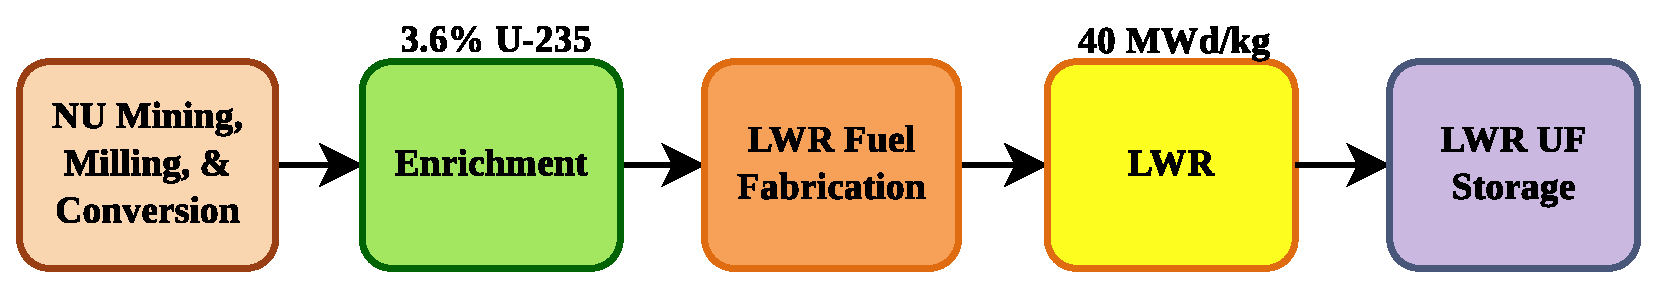
\includegraphics[scale=0.25]{figs/OnceThrough.eps}
    \end{center}

\FromSlide{3}
    \item These base cases are very well studied.

\FromSlide{4}
    \item However, what is \textbf{\textit{not}} well known is 
        how these sample scenarios are affected by perturbations to their 
        initial physical parameters.
            
\FromSlide{1}
\end{itemize}

\FromSlide{5}
\begin{center}
``\textit{Do our parameter choices really give us the `best' solution?}''
\end{center}

\end{slide}}





% Motivation
\begin{slide}{Motivation}
\begin{center}
\begin{figure}
\caption{Physics Modeled versus Execution Time}
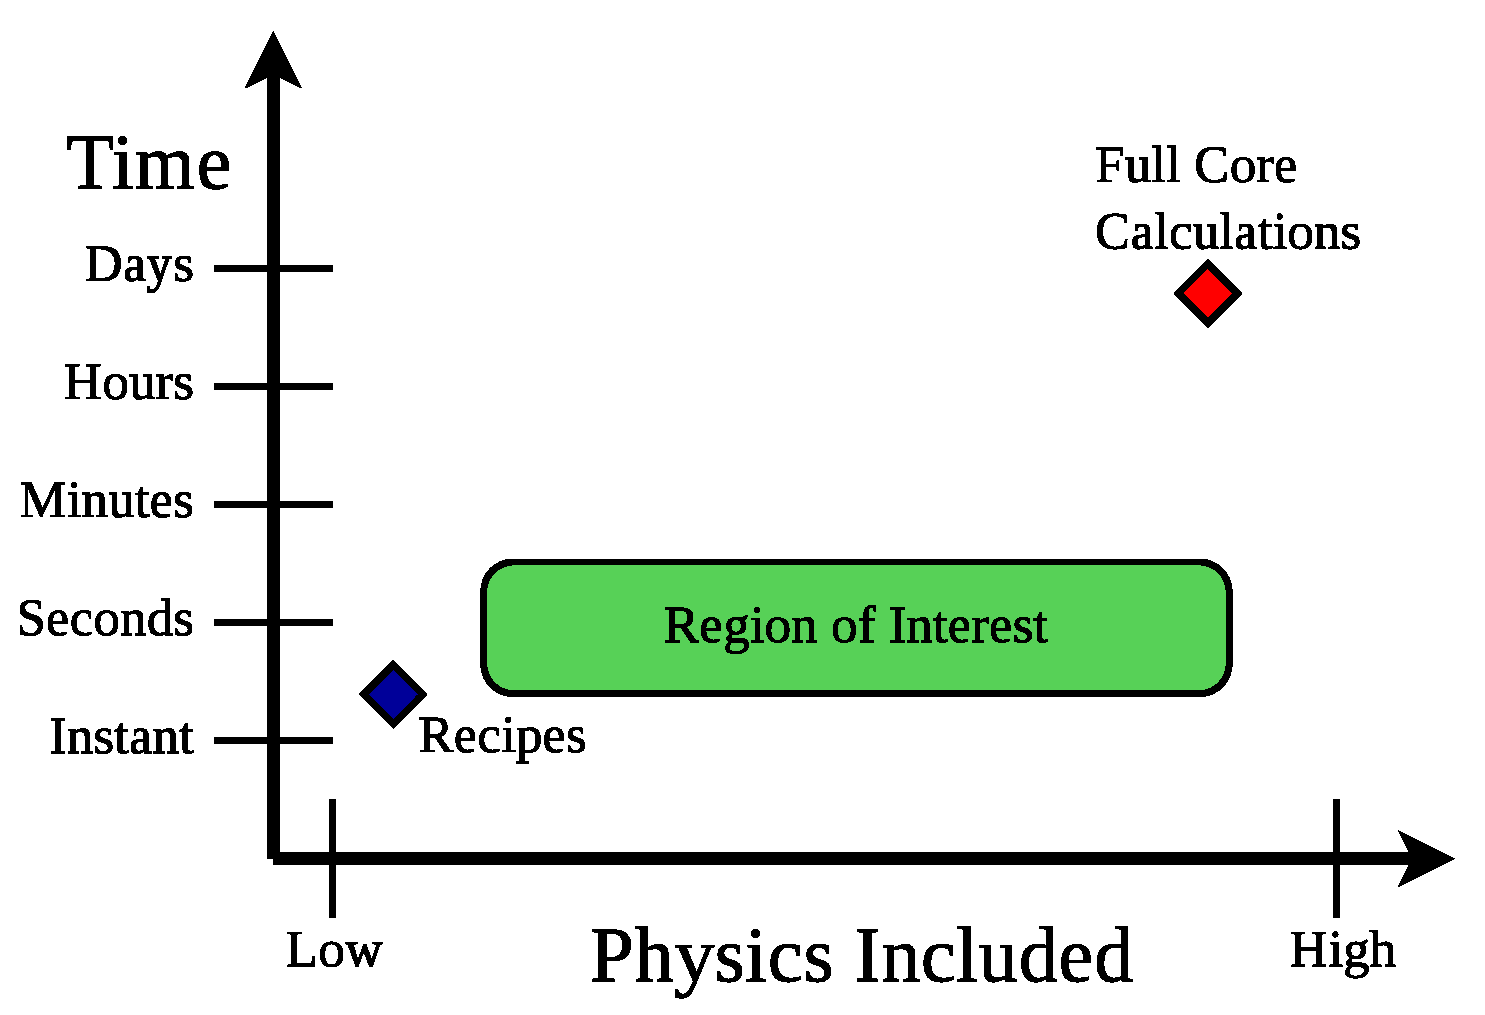
\includegraphics[scale=0.35]{figs/physics_vs_exec_time.eps}
\end{figure}
\end{center}
\end{slide}




% Motivation
\begin{slide}{Motivation}
\small \underline{Basic Fuel Cycle Schema:}
\begin{center}
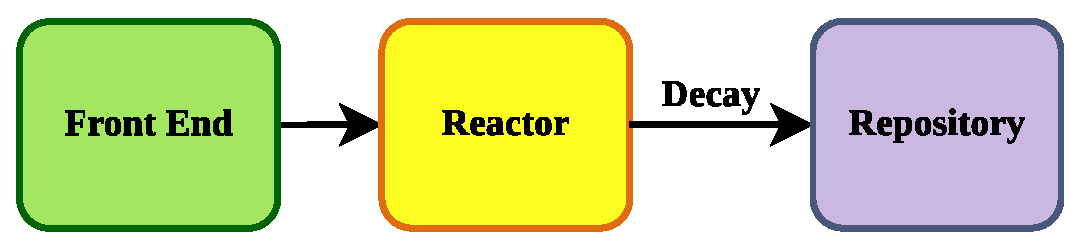
\includegraphics[scale=0.5]{figs/basic_nfc_schema.eps}
\end{center}

\underline{Modeling Approaches:} \small
\begin{center}
\begin{tabular}{lccc}
\textit{Component}                  & \textit{Recipes}  & \textit{Essential} & \textit{Transport}   \\
\underline{\textbf{Front End:}}     & Recipes           & Physics Models     & Physics Models       \\
\underline{\textbf{Reactor:}}       & Recipes           & Rapid Burnup Code  & Neutron Transport    \\
\underline{\textbf{Repository:}}    & Curve Fits        & Rapid Code         & Neutron Transport    \\
\end{tabular}
\end{center}
\end{slide}





% Motivation
\overlays{2}{
\begin{slide}{Motivation}
\FromSlide{1}
\begin{itemize}
    \item Investigating the region of interest may provide a 
        \textit{transformative} amount of fuel cycle data.  

\FromSlide{2}
    \item However, this requires an entirely new spectrum of tools.

\FromSlide{1}
\end{itemize}


\FromSlide{2}
\setcounter{figure}{1}
\begin{center}
\begin{figure}
\caption{Fuel Cycle Stack}
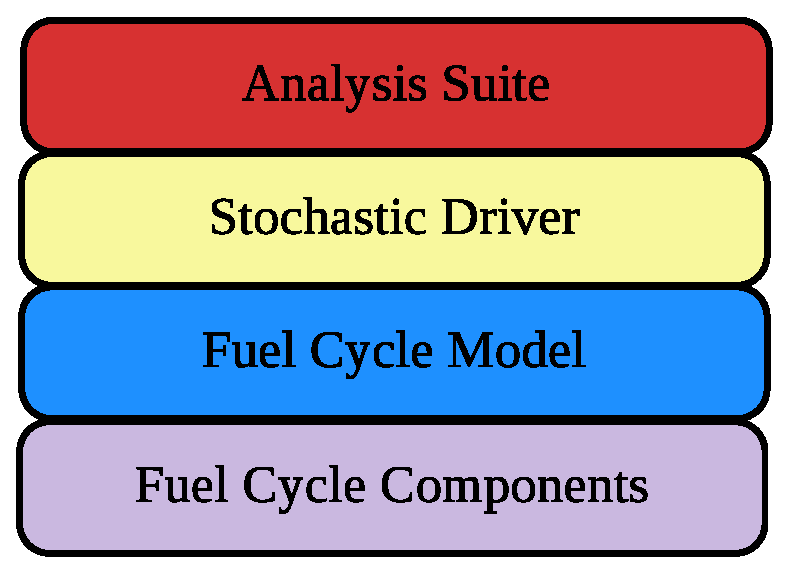
\includegraphics[scale=0.35]{figs/fc_stack.eps}
\end{figure}
\end{center}

\end{slide}}



% Definition
\begin{slide}{Definition}
\vspace{3.0cm}
\begin{center}
\textit{Essential physics} models remain physically valid under perturbations
in the locality of the region that they are defined and do not compute
extraneous parameters.  
\end{center}
\end{slide}




% A Path Forward
\overlays{4}{
\begin{slide}{A Path Forward}
\FromSlide{1}
\begin{itemize}
    \item Develop a set of fuel cycle component models which 
        preserve basic physics (largely focused on a one-enegy 
        group reactor model, R1G).

\FromSlide{2}
    \item Investigate a categorical set of fuels cycles using
        the above components. (These are largely linear 
        perturbations of previous base-case studies.)

\FromSlide{3}
    \item Extend the fuel cycle model to perturb continuous 
        variables.  This requires a stochastic driving mechanism
        to run.  Moreover, it requires entropy-based measures to
        analyze.

\FromSlide{4}
    \item Model the reactor compoent with 
        multiple energy groups (RMG).  This enables the study 
        of reactors and fuel cycles forbidden in the R1G regime.

\FromSlide{1}
\end{itemize}
\end{slide}}




% R1G
\begin{slide}{R1G}
\vspace{3.5cm}
\begin{center}
\Large
One-Group Reactor Model
\end{center}
\end{slide}





% R1G
\begin{slide}{R1G}
\begin{center}
\begin{figure}
\caption{Reactor Model [1]}
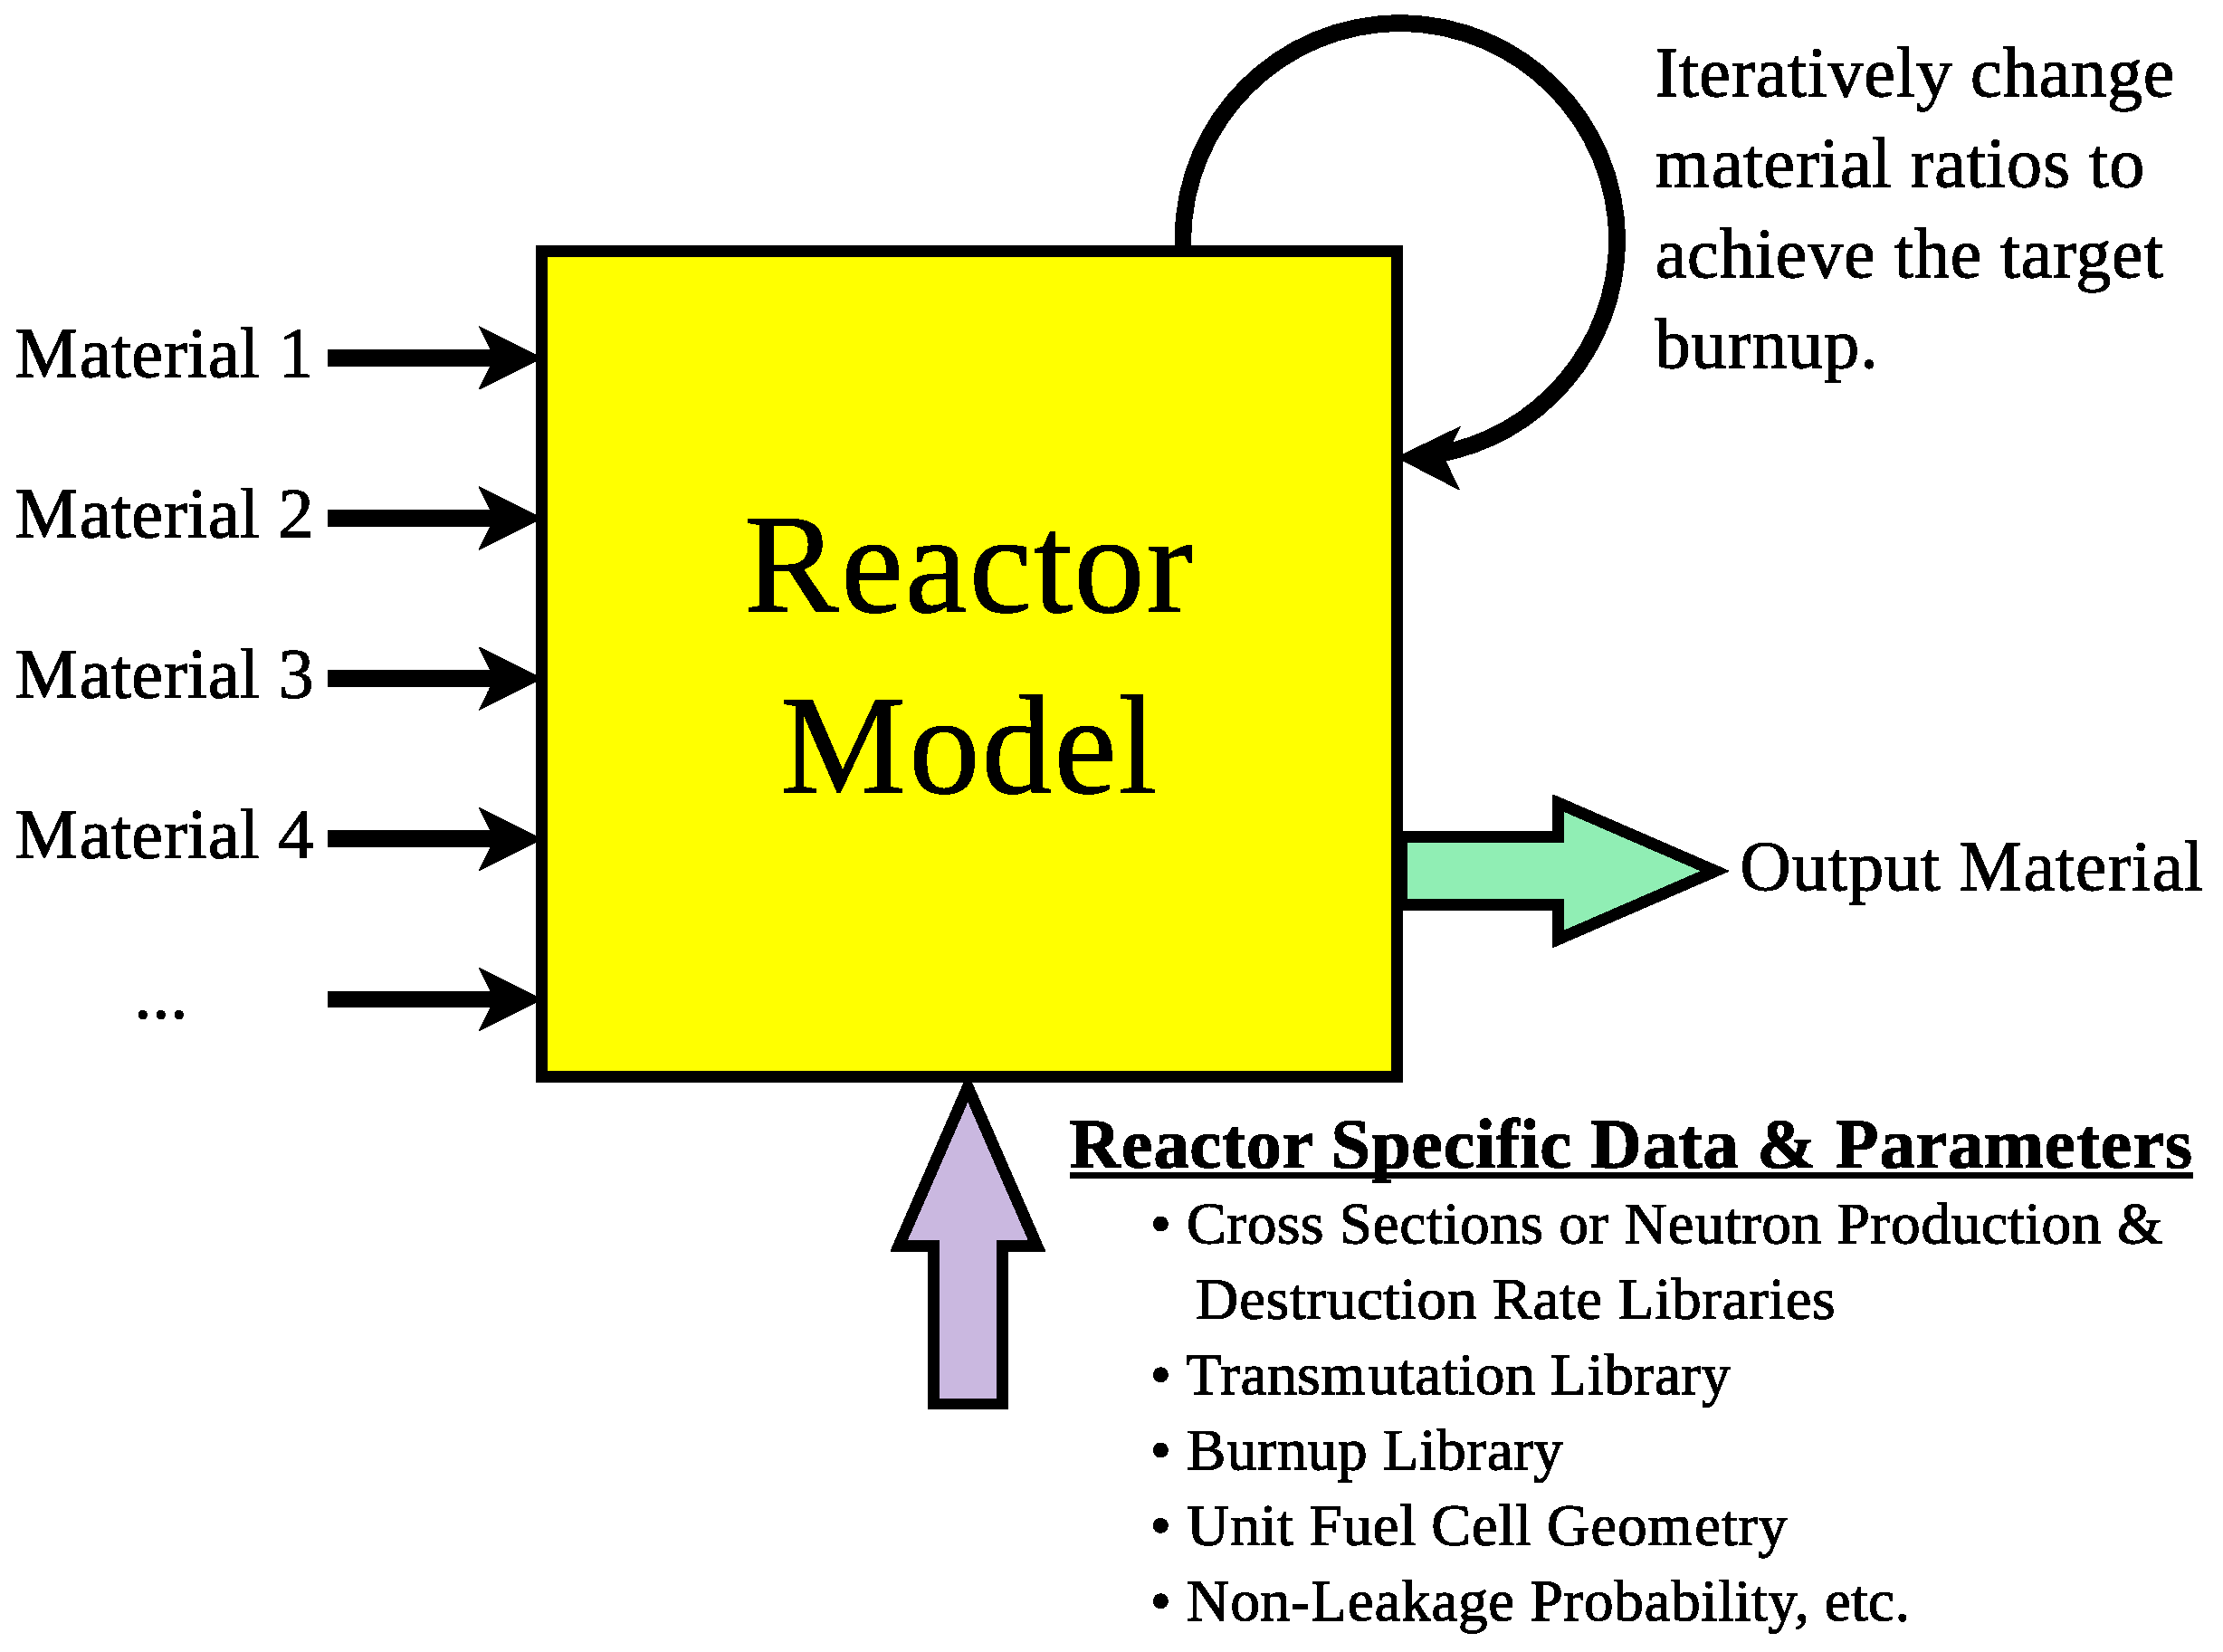
\includegraphics[scale=0.20]{figs/reactor_model.eps}
\end{figure}
\end{center}
\end{slide}



% R1G Notation
\begin{slide}{R1G Notation}
\vspace{0.75cm}
\begin{center}
\begin{table}
\caption{One-Group Reactor Symbols}
\tiny
\begin{tabular}{|l|c|c|}
\hline
\textbf{Name} & \textbf{Symbol} & \textbf{Units} \\
\hline
Fluence & $F = \int_0^t \phi dt^\prime = \phi \int_0^t dt^\prime = \phi \times t \cdot \frac{24 \cdot 3600 \cdot 10^3}{10^{24}}$ & [n/kb] \\
Nuclide Subscript & $i$ (or $j$) & [1/kg\subscript{$i$}] \\
Region Superscript & $Q$ & [unitless] \\
Mass Weights & $m_i^Q = \frac{N_i^Q}{N_{\mbox{IHM}}} = \frac{n_i^Q A_i}{A_{\mbox{IHM}}} \cdot \frac{\rho^Q\cdot\mbox{MW}^F}{\rho^F\cdot\mbox{MW}^Q} \frac{V^Q}{V^F}$ & [kg$_i^Q$/kgIHM] \\
Burnup & $\mbox{BU}(F) = \sum_i m_i^F \cdot \mbox{BU}_i(F)$ & [MWd/kgIHM] \\
Prod \& Des Rates & $p_i(F), d_i(F)$ & [n/s/flux/kg$_i$]\\ 
Transmutation Matrix & $T_{ij}(F)$ & [kg$_j$/kg$_i$] \\
Multiplication Factor & $k(F) = \frac{P(F)}{D(F)}$ & [unitless] \\
\hline
\end{tabular}
\end{table}
\end{center}
\end{slide}





% R1G
\overlays{2}{
\begin{slide}{R1G}
\FromSlide{1}
\begin{center}
Starting with ORIGEN generated fluence-dependent, nuclide specific data, we know:

\setcounter{figure}{3}
\begin{figure}
\subfloat[prod \& des rates,]{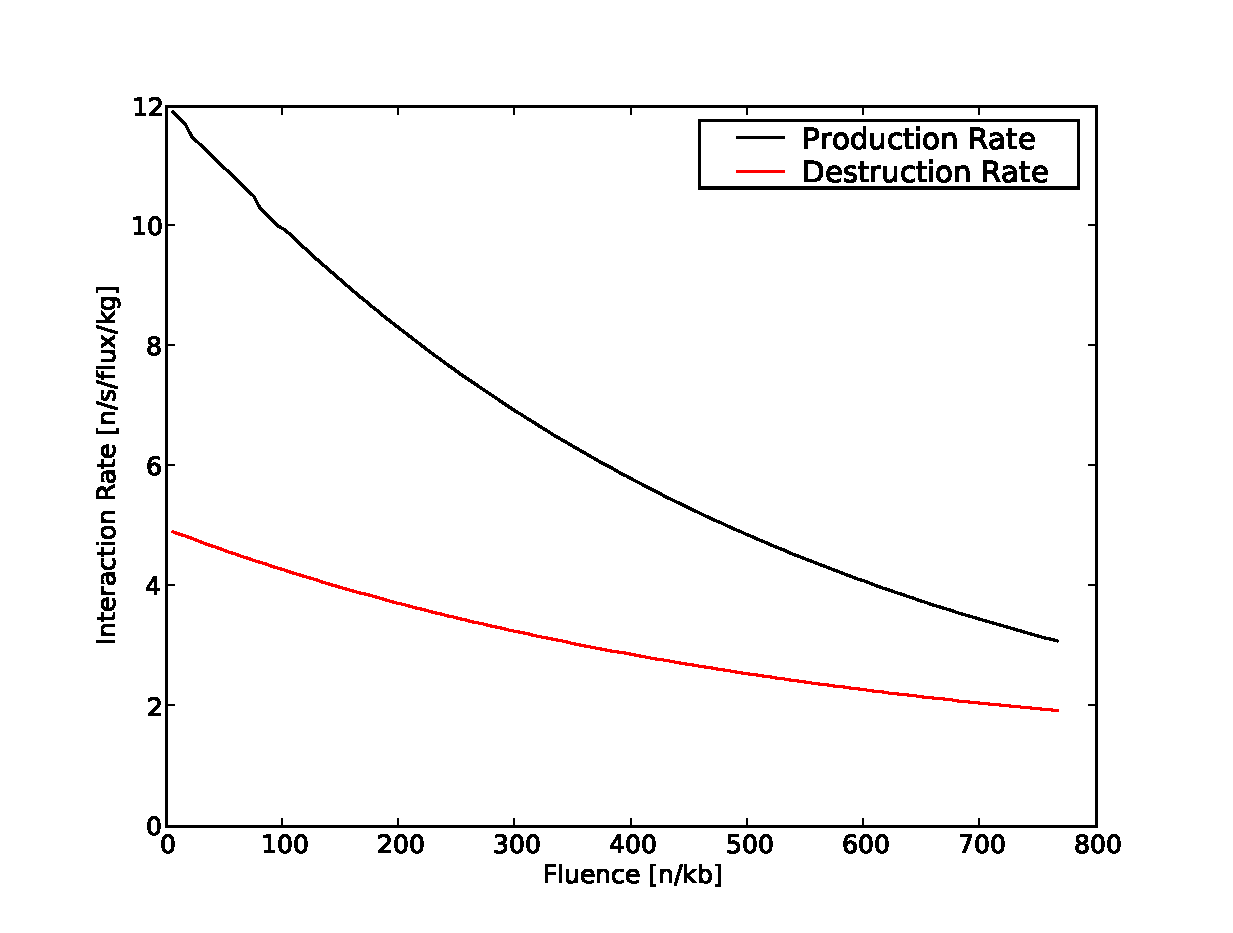
\includegraphics[scale=0.21]{../one_group_method/figs/Fig02.eps}}
\subfloat[burnups,]{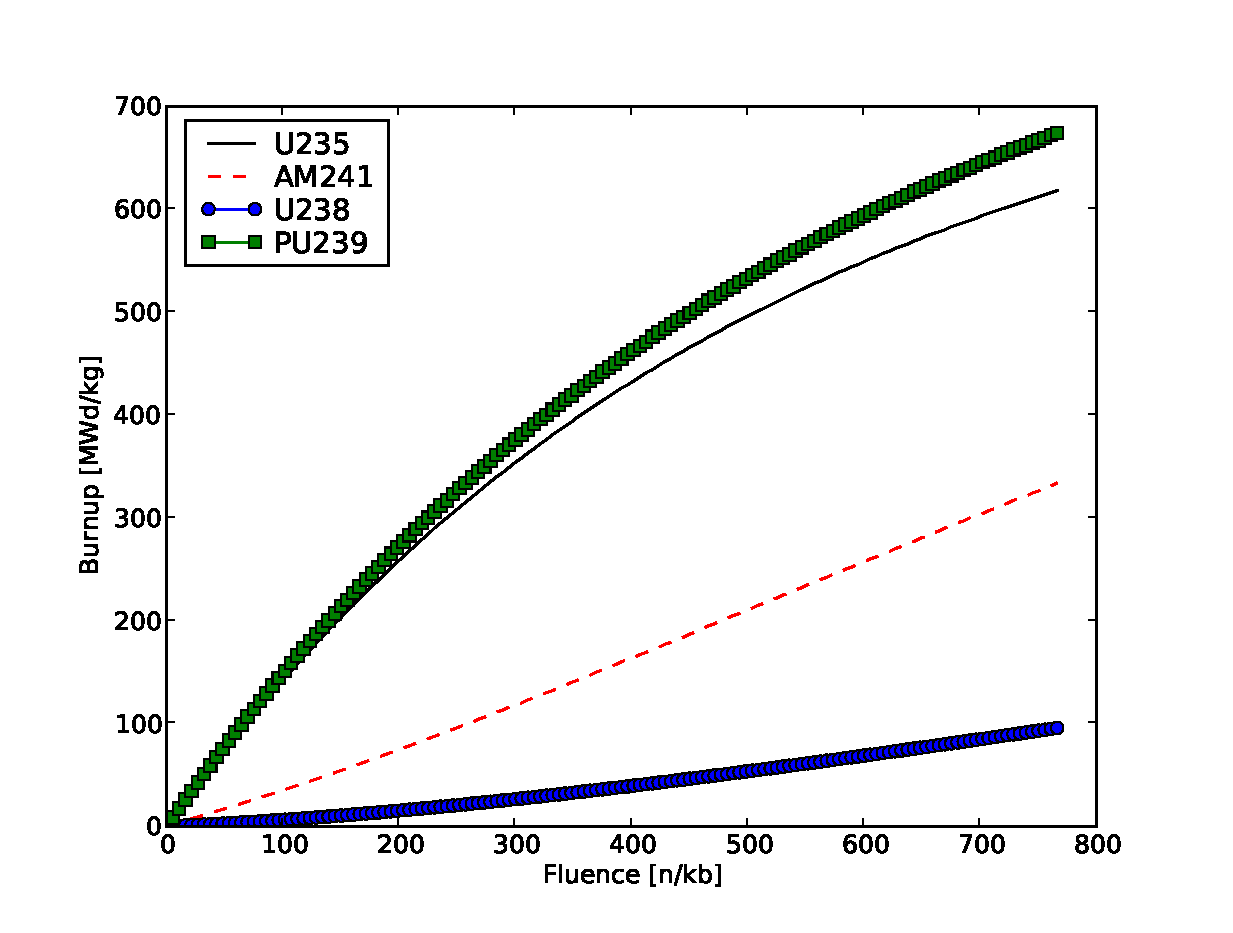
\includegraphics[scale=0.21]{../one_group_method/figs/Fig03.eps}}
\subfloat[transmutation matrices.]{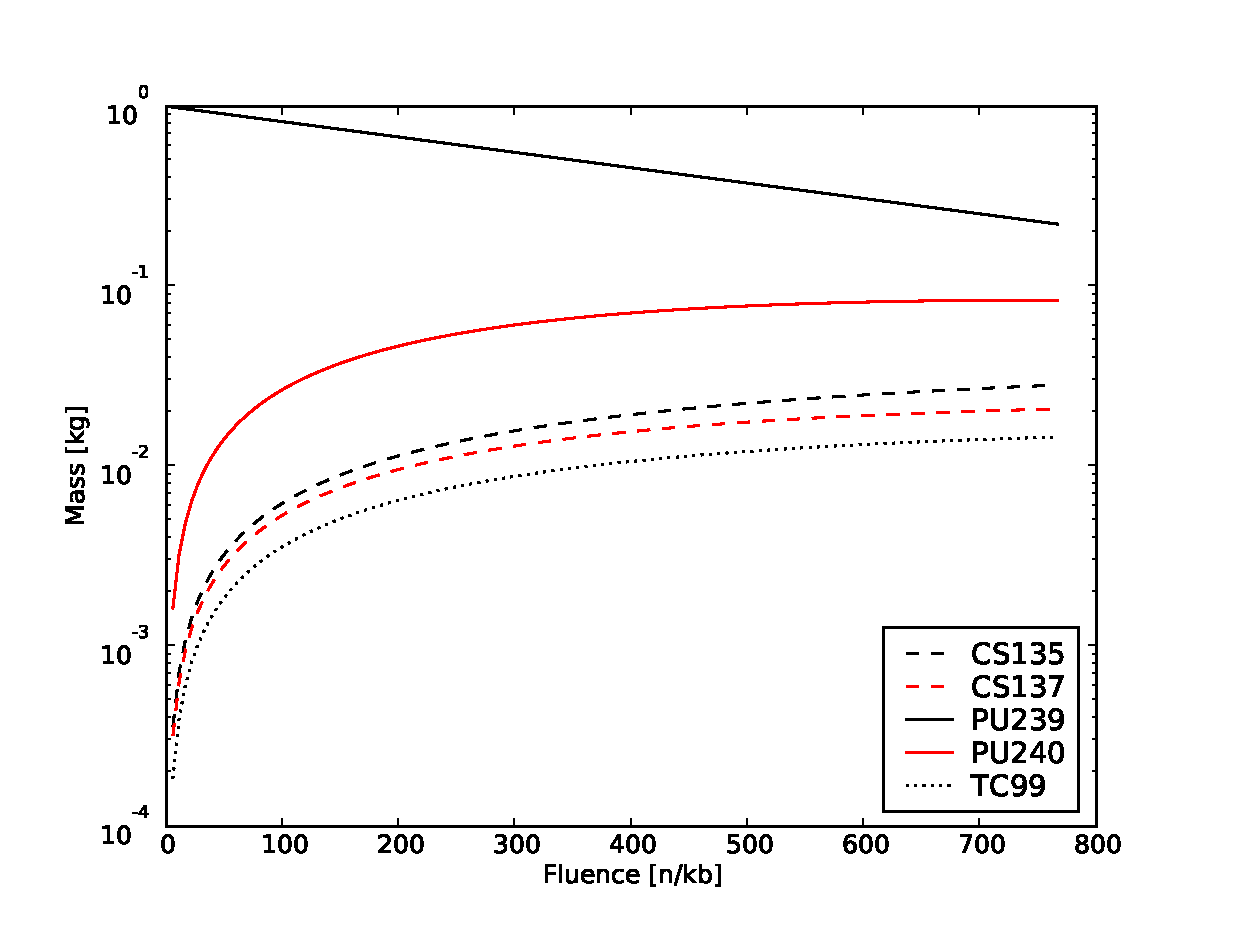
\includegraphics[scale=0.21]{../one_group_method/figs/Fig01.eps}}
\caption{Reactor Data Library (for FR \nuc{Pu}{239})}
\end{figure}

\end{center}

\FromSlide{2}
\footnotesize
To obtan a specific reactor, the above data must be folded together.
\end{slide}}



% R1G Library Collapse
\overlays{4}{
\begin{slide}{R1G Library Collapse}
\FromSlide{1}
\begin{itemize}
    \item Collapsing a general library down is the central calculation of 
        the one-group reactor model.

\FromSlide{2}
    \item Using a two-region fuel pin cell model, denote the mass weight of each initial 
        isotope $i$ in the fuel as $m^F_i$ and the in the coolant as $m^C_i$.

\FromSlide{3}
    \item Then, a mass-weighted linear combination of all of the library
        parameters computes the full-core values.

\FromSlide{4}
    \item For example, 

        \[ P(F) = P_{NL} \cdot p^F(F) = P_{NL} \sum^I_i m^F_i \cdot p^F_i(F) \]
\FromSlide{1}
\end{itemize}
\end{slide}}





% R1G
\begin{slide}{R1G}
\begin{center}
\begin{figure}
\caption{Linearly Weighted Fast Reactor Data}
\subfloat[Burnup]{\includegraphics[scale=0.31]{../one_group_method/figs/Fig05.eps}}
\subfloat[Multiplication Factor]{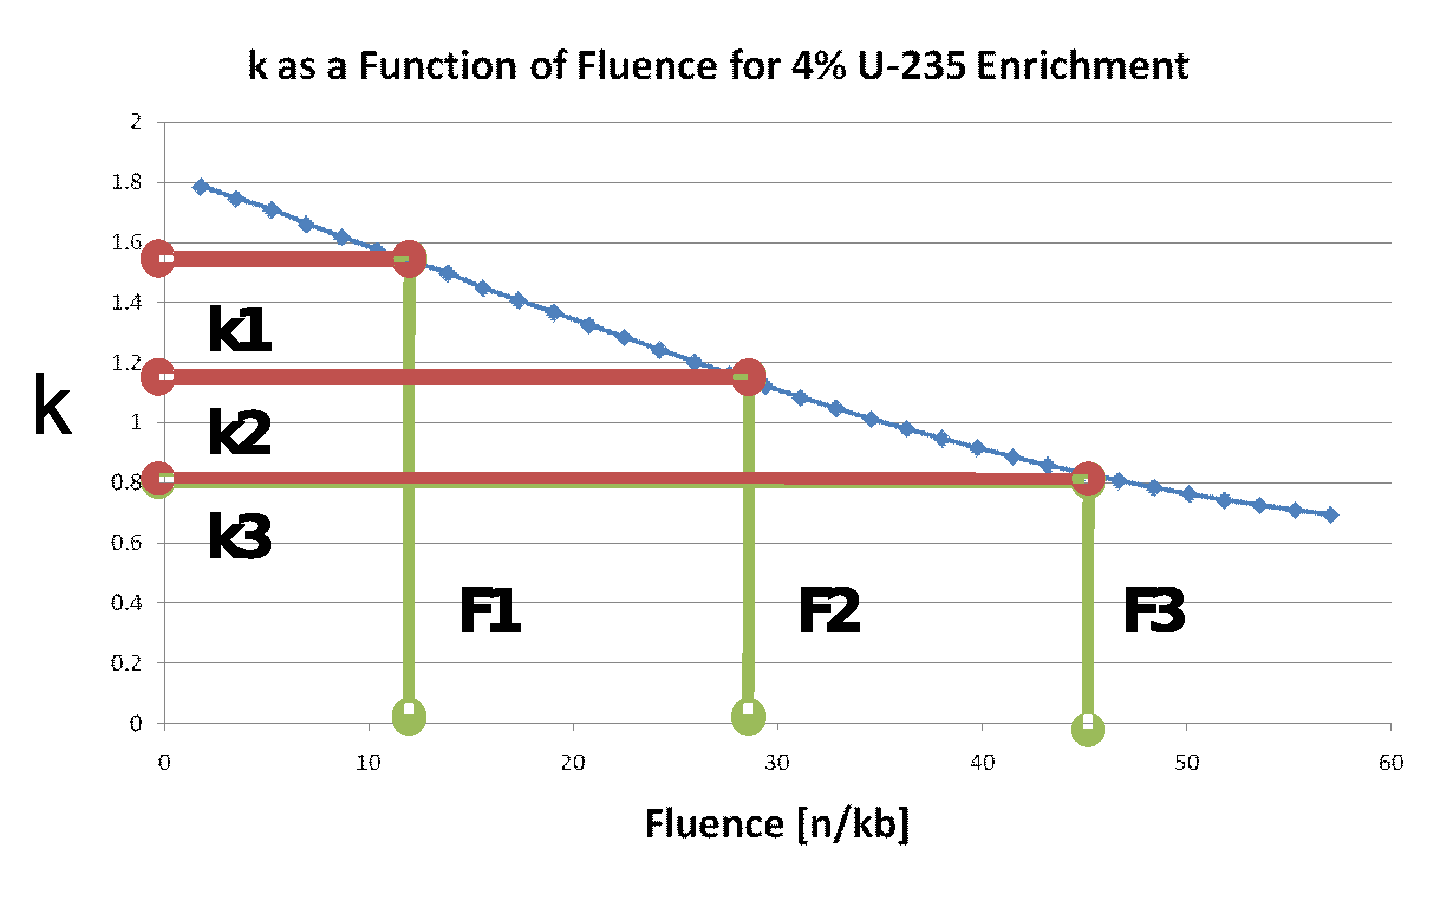
\includegraphics[scale=0.31]{../one_group_method/figs/Fig06.eps}}
\end{figure}
\end{center}
\end{slide}




% R1G 
\overlays{3}{
\begin{slide}{R1G}
\FromSlide{1}
\begin{minipage}[t]{0.49\textwidth}
\setcounter{figure}{5}
\begin{center}
\begin{figure}
\caption{Fast Reactor\\ Discharge Composition}
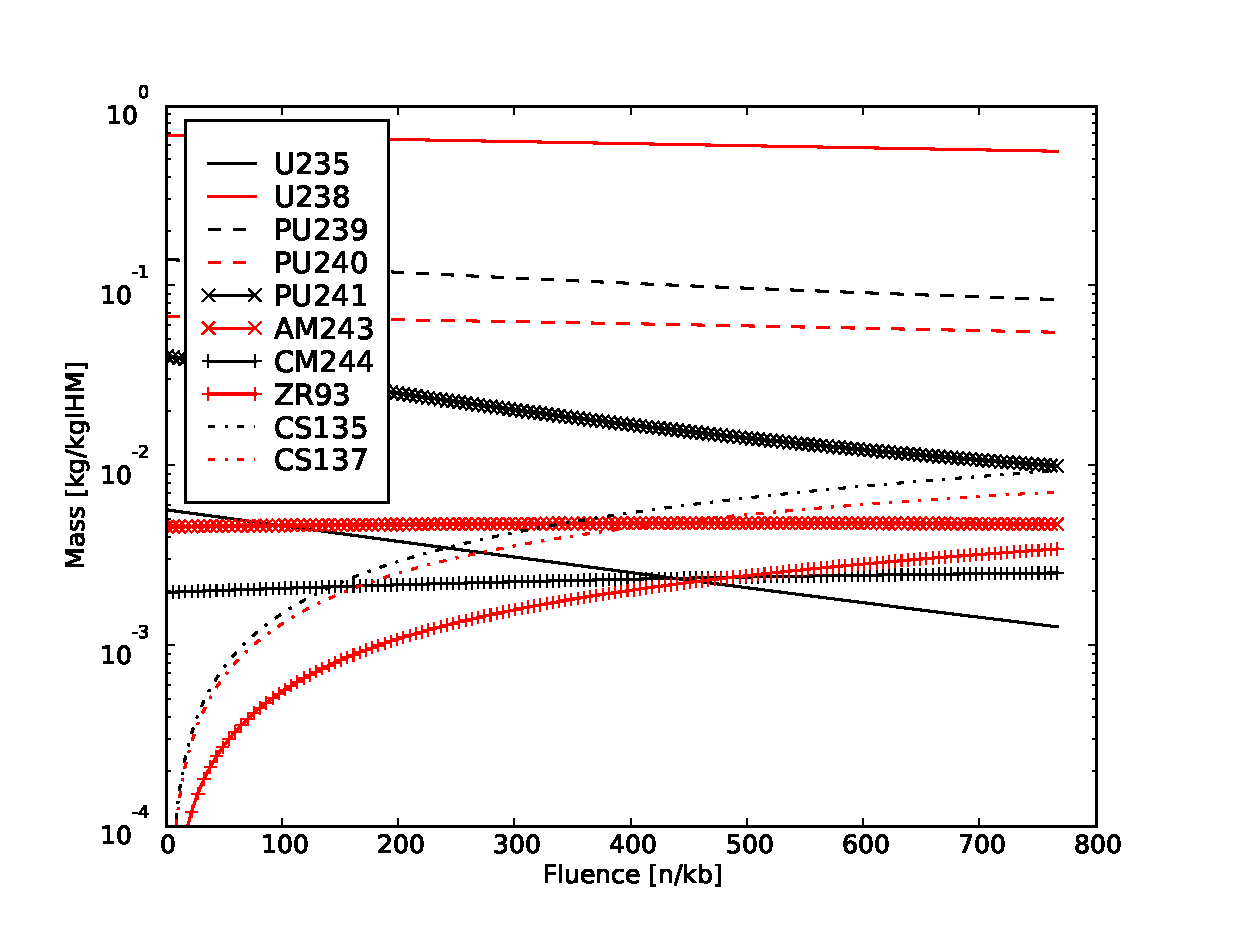
\includegraphics[scale=0.3]{../one_group_method/figs/Fig07.eps}
\end{figure}
\end{center}
\end{minipage}
\begin{minipage}[t]{0.49\textwidth}
\small
\begin{itemize}
    \item The transmutation matrices may be similarly weighted by inital composition.

\FromSlide{2}
    \item From the criticality calculation above we also know the discharge fluence, Fd [n/kb].

\FromSlide{3}
    \item Therefore the used fuel composition is known by taking the nuclide mass weights at 
            Fd in Figure 6.

\FromSlide{1}
\end{itemize}
\end{minipage}
\end{slide}}




% R1G Benchmark
\begin{slide}{R1G Benchmark}
\tiny
\begin{table}[htbp]
\begin{center}
\caption{LWR Benchmark to OECD Burnup Credit [2]}
\begin{tabular}{|l|c|c|c|c|}
\hline
\textbf{Nuclide} & \textbf{OECD [2] [w/o]} & \textbf{$\sigma$ of OECD [\%]} & \textbf{Results [w/o]} & \textbf{\% Difference} \\
\hline
\nuc{U}{234}     & 0.0178  & 9.0  & 0.0184  & +3.6  \\
\nuc{U}{235}     & 0.8001  & 8.1  & 0.7079  & -11.5 \\
\nuc{U}{236}     & 0.4840  & 2.6  & 0.4781  & -1.2  \\
\nuc{U}{238}     & 93.3333 & 0.2  & 93.6109 & +0.3  \\
\nuc{Np}{237}    & 0.0614  & 9.4  & 0.0584  & -5.0  \\
\nuc{Pu}{238}    & 0.0226  & 13.9 & 0.0185  & -18.1 \\
\nuc{Pu}{239}    & 0.5991  & 7.1  & 0.5104  & +14.8 \\
\nuc{Pu}{240}    & 0.2389  & 5.3  & 0.2591  & +8.5  \\
\nuc{Pu}{241}    & 0.1636  & 6.9  & 0.1445  & -11.7 \\
\nuc{Pu}{242}    & 0.0602  & 8.4  & 0.0563  & -6.5  \\
\nuc{Am}{241}    & 0.0047  & 5.3  & 0.0032  & -30.8 \\
\nuc{Am}{243}    & 0.0148  & 10.4 & 0.0116  & -21.3 \\
\hline
\end{tabular}
\end{center}
\end{table}
\end{slide}



% R1G Bechmark Notes
\overlays{2}{
\begin{slide}{R1G Bechmark Notes}
\FromSlide{1}
\begin{itemize}
    \item This benchmark compares an OECD study for a 40 MWd/kgIHM burn with no cooling.

    \item This result shows the R1G matches the burnup credit to within two standard 
        deviations for most actinides.

\FromSlide{2}
    \item \nuc{Am}{241} is the only nuclide showing a relatively higher departure.

    \item This sepcies is formed through \nuc{Pu}{241} decay.

    \item \nuc{Am}{241} would thus match better if a constant flux or 
        if zero reloading times were not assumed.

\FromSlide{1}
\end{itemize}
\end{slide}}




% R1G Fuel Cycle Example: RU
\overlays{3}{
\begin{slide}{R1G Fuel Cycle Example: RU}
\FromSlide{1}
\begin{minipage}[t]{0.49\textwidth}
\small
\begin{itemize}
    \item Recyclable Uranium (RU) is obtained by reprocessing used fuel.

\FromSlide{2}
    \item The RU fuel cycle was split into three energy-equivelent bases which 
        were then compared.

\FromSlide{3}
    \item All options share a common front \& back end fuel cycle.  Therefore
        cost-benefit analyses focus on the differening components.

\FromSlide{1}
\end{itemize}
\end{minipage}
\begin{minipage}[t]{0.49\textwidth}
\setcounter{figure}{6}
\begin{center}
\begin{figure}
\caption{RU Fuel Cycles}
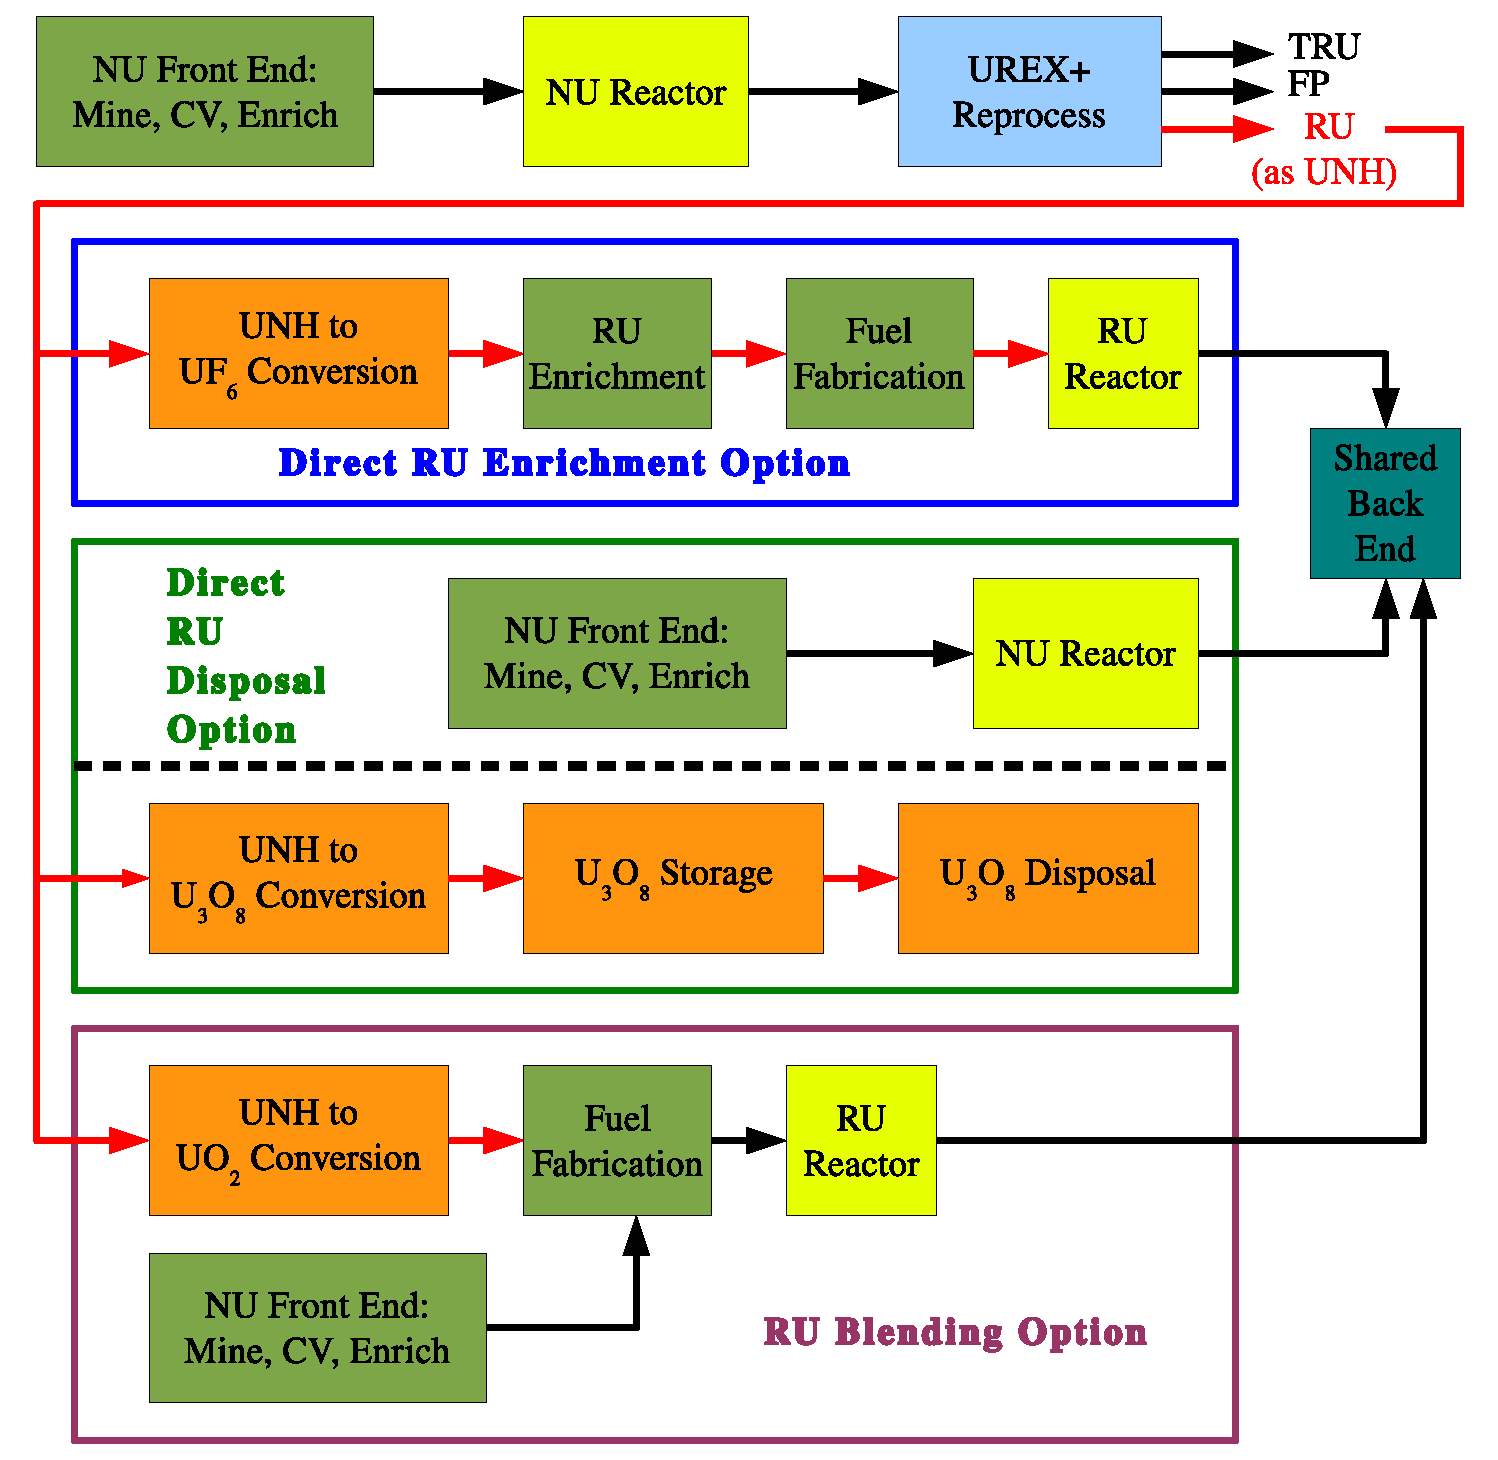
\includegraphics[scale=0.25]{../one_group_method/figs/Fig08.eps}
\end{figure}
\end{center}
\end{minipage}
\end{slide}}





% R1G Fuel Cycle Example: RU
\overlays{4}{
\begin{slide}{R1G Fuel Cycle Example: RU}
\FromSlide{1}
\begin{minipage}[t]{0.49\textwidth}

\setcounter{figure}{7}
\begin{center}
\begin{figure}
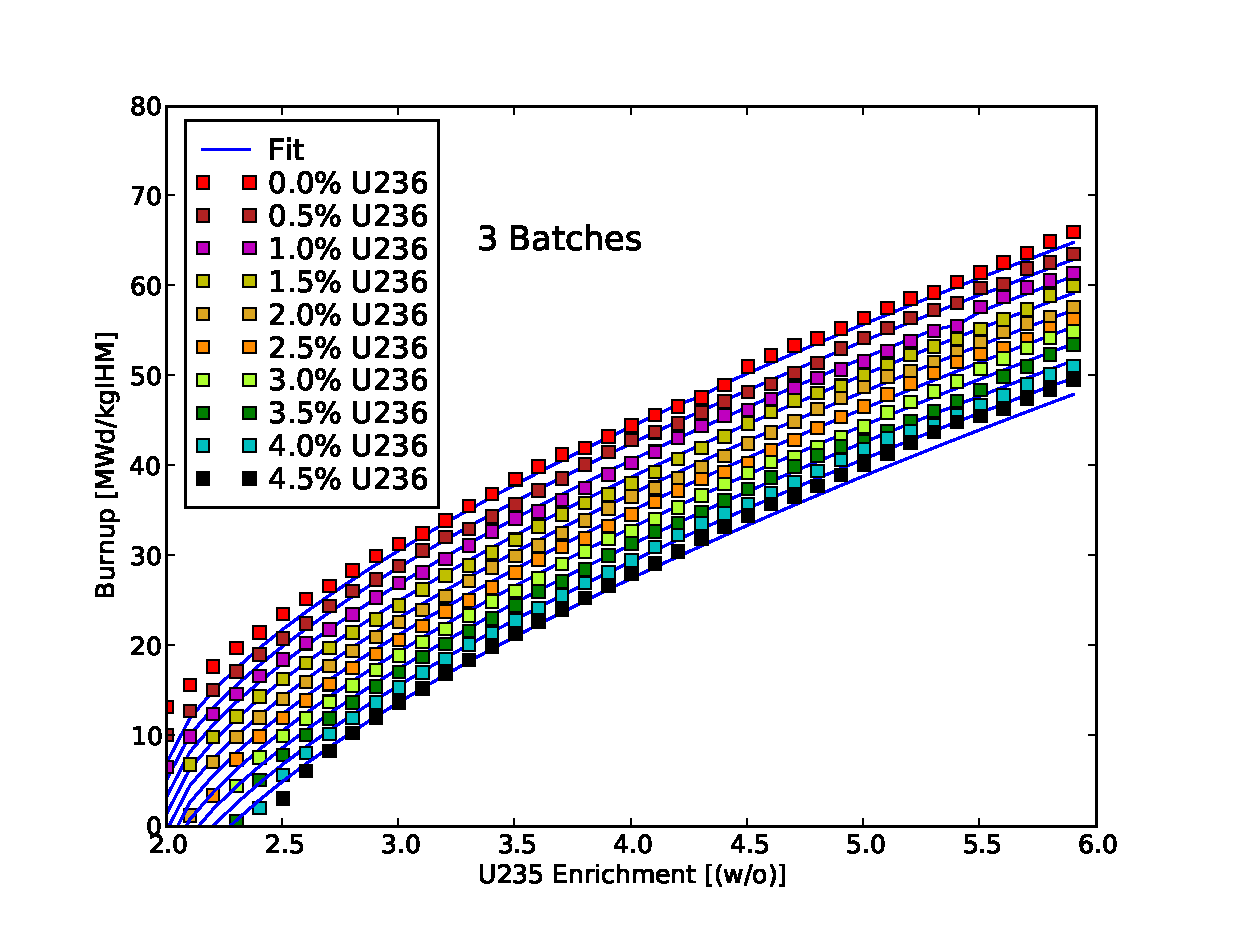
\includegraphics[scale=0.32]{../one_group_method/figs/Fig14.eps}
\caption{Burnup Model Fit for LWRs}
\end{figure}
\end{center}

\end{minipage}
\begin{minipage}[t]{0.49\textwidth}
\footnotesize
\begin{itemize}
    \item RU utility may be further parameterized as a function of \nuc{U}{235},
        \nuc{U}{236}, and the batch loading scheme.  (Not possible for FRs.)

\FromSlide{2}
    \item In Figure 8, data points were calculated and blue lines represent 
        a best-fit curve.

\FromSlide{3}
    \item The 0\% \nuc{U}{236} curve represents a standard LWR.

\FromSlide{4}
    \item This further reduces the computational load of the R1G while remaining 
        perturbable.

\FromSlide{1}
\end{itemize}
\end{minipage}
\end{slide}}





% R1G Fuel Cycle Example: RU
\begin{slide}{R1G Fuel Cycle Example: RU}
\begin{center}
\begin{figure}
\caption{RU Blend Cycle with Mass Balances}
\includegraphics[scale=0.35]{../one_group_method/figs/Fig17.eps}
\end{figure}
\end{center}
\end{slide}





%
% OMG next section
%

% Fuel Cycle Sensitivity Study
\begin{slide}{Sensitivity Study}
\vspace{3.5cm}
\begin{center}
\Large
Fuel Cycle Sensitivity Study
\end{center}
\end{slide}





% Sensitivity Methodology Overview
\overlays{4}{
\begin{slide}{Sensitivity Methodology Overview}
\FromSlide{1}
\begin{itemize}
    \item Here, the system-wide impact of physical parameter perturbations is quantified.

\vspace{0.5cm}
\FromSlide{2}
    \item This is done by looking for linear, 1D sensitivity coefficients for each parameter
        to the \underline{repository capacity} response, measured in [PWh].   

\vspace{0.5cm}
\FromSlide{3}
    \item Denote these sensitivity coefficients as $S_x$ for a small change in an input parameter $x$.

\vspace{0.5cm}
\FromSlide{4}
    \item Sensitivity coefficients are presented for 10\% 
        changes in $x$ from assumed base-case values.

\FromSlide{1}
\end{itemize}
\end{slide}}







% Sensitivity Methodology Overview
\overlays{5}{
\begin{slide}{Sensitivity Methodology Overview}
\FromSlide{1}
\begin{itemize}
\FromSlide{1}
    \item The basic algorithm is as follows:

\tiny
\FromSlide{2}
        \begin{enumerate}
            \item For each input parameter $x$, change its base-case value $x_0$ by $\pm10\%$.
                \[ x \to (1 \pm 0.1)x_0 \]

            \FromSlide{3}
            \item If $x$ is a separation efficiency (SE), instead perturb by $\pm$ ``one nine''
                worth of separations.
                \[ x = 0.999 \to x \in \{0.99, 0.9999\} \]

            \FromSlide{4}
            \item Meanwhile, maintain all other parameters ($y, z, \ldots$) at their
                base-case values.
                \[ y, z, \ldots \to y_0, z_0, \ldots \]    

            \FromSlide{5}
            \item Calculate the new repository capacity response, $R$, by the perturbed cycle and record 
                the sensitivity as the percent change from the base-case response, $R_0$.
                \[ S_{\pm x} = \left(\frac{R}{R_0} - 1\right) \times 100 \]

        \FromSlide{2}
        \end{enumerate}

\FromSlide{1}
\end{itemize}
\end{slide}}



% Fuel Cycle
\overlays{2}{
\begin{slide}{Fuel Cycle}
\FromSlide{1}
\begin{itemize}
    \item The essential physics models from before were
        used it to study a Fast Reactor (FR), Light
        Water Reactor (LWR) symbiotic scenario 
        analogous to Scheme 3a of a 2006 OECD report [3].
\end{itemize}

\FromSlide{2}
\setcounter{figure}{9}
\begin{center}
\begin{figure}
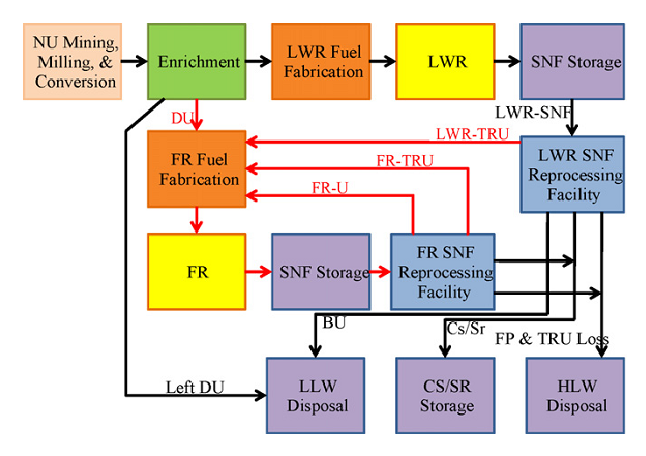
\includegraphics[scale=0.2]{../one_group_method/figs/Fig09.eps}
\caption{LWR-FR Fuel Cycle}
\end{figure}
\end{center}
\end{slide}}




% Fuel Cycle
\overlays{3}{
\begin{slide}{Fuel Cycle}
\FromSlide{1}
\small
With perturbable components, over 30 independent physical 
parameters may be adjusted in the fuel cycle.
\FromSlide{2}
\setcounter{figure}{10}
\begin{figure}
\begin{center}
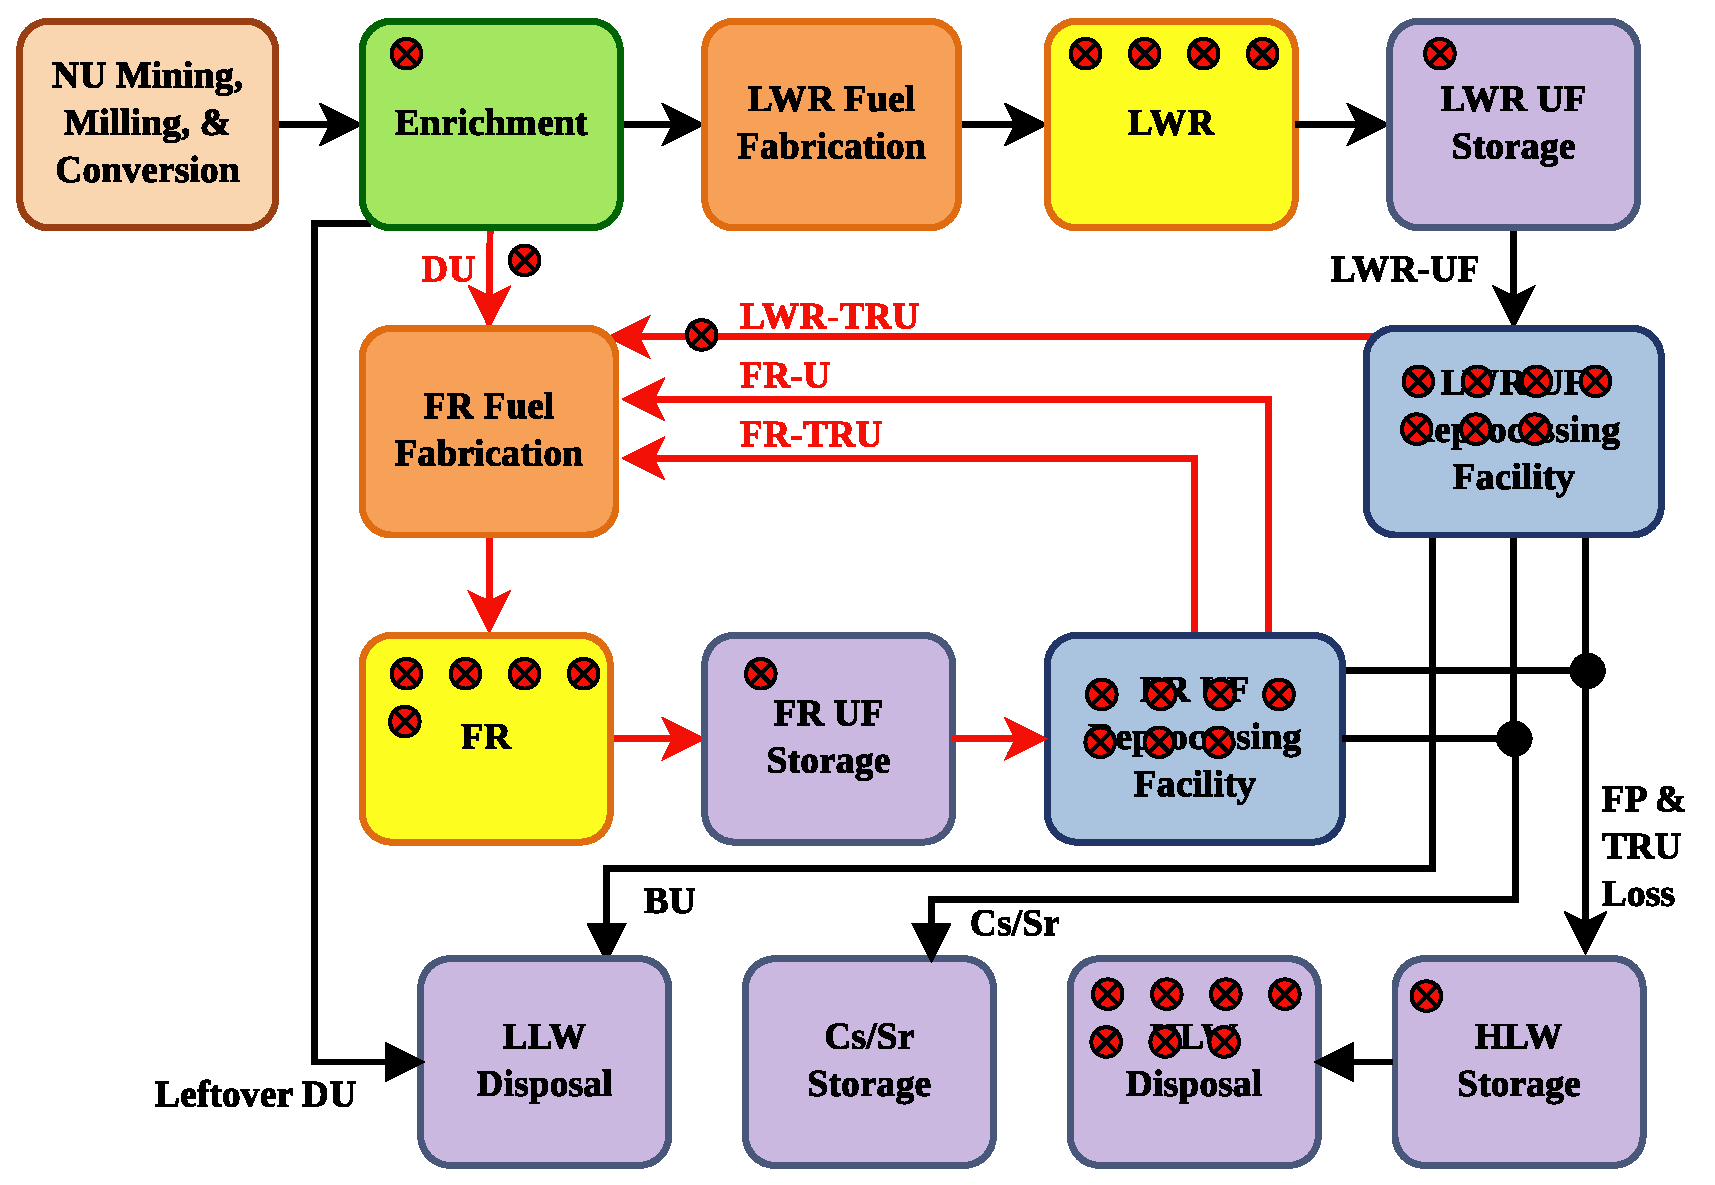
\includegraphics[scale=0.2]{figs/LWR_FR_FC_knobs.eps}
\caption{LWR-FR Cycle with Parameters}
\end{center}
\end{figure}
\FromSlide{3}
\small
Sensitivity results are computed from equilibrium values derived from 
a full treatment of the preceeding, transient cycles.
\end{slide}}




% Base Case Parameter Definition
\begin{slide}{Base Case Parameter Definition}
\tiny
\begin{center}
\begin{tabular}{|l||c|c|}
\hline
\textbf{Input Parameter $x$} & \textbf{Value} & \textbf{Units} \\
\hline
LWR Burnup & 50.0 & MWd/kgIHM \\
\hline
LWR Fuel to Moderator Ratio & 0.301 & \\
\hline
LWR UF Storage Time & 60 & years \\
\hline
SE of U from LWR UF & 0.999 & \\
\hline
SE of NP from LWR UF & 0.999 & \\
\hline
SE of PU from LWR UF & 0.999 & \\
\hline
SE of AM from LWR UF & 0.999 & \\
\hline
SE of CM from LWR UF & 0.999 & \\
\hline
SE of CS from LWR UF & 0.999 & \\
\hline
SE of SR from LWR UF & 0.999 & \\
\hline
FR Burnup & 140.0 & MWd/kgIHM \\
\hline
FR TRU Conversion Ratio & 0.50 & \\
\hline
Max Fraction of Lanthanide in FR Fuel & 0.0005 & Atoms/TRU Atom \\
\hline
FR UF Storage Time & 3 & years \\
\hline
Storage Before Disposal & 50 & years \\
\hline
\end{tabular}
\end{center}
\end{slide}



% Base Case Parameter Definition
\begin{slide}{Base Case Parameter Definition}
\tiny
\begin{center}
\begin{tabular}{|l||c|c|}
\hline
\textbf{Input Parameter $x$} & \textbf{Value} & \textbf{Units} \\
\hline
SE of U from FR UF & 0.999 & \\
\hline
SE of NP from FR UF & 0.999 & \\
\hline
SE of PU from FR UF & 0.999 & \\
\hline
SE of AM from FR UF & 0.999 & \\
\hline
SE of CM from FR UF & 0.999 & \\
\hline
SE of CS from FR UF & 0.999 & \\
\hline
SE of SR from FR UF & 0.999 & \\
\hline
Density of Host Rock & 2580 & kg/m\superscript{3} \\
\hline
Specific Heat of Host Rock & 840 & J/kg-K \\
\hline
Thermal Conductivity of Host Rock & 1.626 & W/m-K \\
\hline
Heat Loss Factor During Ventilation  & 0.7 & \\
\hline
Drift diameter & 5.5 & m \\
\hline
Ventilation System On Time & 50 & years \\
\hline
Ambient Environment Temperature & 20 & C \\
\hline
Distance Between Drifts & 81 & m \\
\hline
\end{tabular}
\end{center}
\end{slide}






% Fuel Cycle Benchmark
\begin{slide}{Fuel Cycle Base Case Benchmark}
\tiny
\begin{center}
\begin{tabular}{|l||c||c|c||c|c|}
\hline
\textbf{Scheme 3a}     & \textbf{NEA [3]} & \textbf{Model\superscript{1}} & \textbf{\% Diff} & \textbf{Model\superscript{2}} & \textbf{\% Diff} \\
\hline
Electricity Share: LWR & 0.632       & 0.619459             & -2.0244 & 0.634907             & +0.4579 \\
\hline
Electricity Share: FR  & 0.368       & 0.380541             & +3.2955 & 0.365093             & -0.7962 \\
\hline
FR UF: U               & 0.698       & 0.713806             & +2.2143 & 0.715224             & +2.4082 \\
\hline
FR UF: NP              & 0.0065      & 0.00661961           & +1.8070 & 0.00685174           & +5.1335 \\
\hline
FR UF: PU              & 0.266       & 0.248059             & -7.2327 & 0.248319             & -7.1204 \\
\hline
FR UF: AM              & 0.02        & 0.0226796            & 11.8152 & 0.0217317            & +7.9687 \\
\hline
FR UF: CM              & 0.0098      & 0.00883517           & -10.920 & 0.00787319           & -24.4730\\
\hline
HLW: U                 & 0.013324    & 0.0132681            & -0.4213 & 0.0134448            & +0.8984 \\
\hline
HLW: NP                & 2.26542E-05 & 2.4079E-05           & +5.9173 & 2.41083E-05          & +6.0316 \\
\hline
HLW: PU                & 0.000704797 & 0.000658893          & -6.9668 & 0.000632361          & -11.4548\\
\hline
HLW: AM                & 5.03426E-05 & 5.63068E-05          & 10.5923 & 5.12344E-05          & +1.7405 \\
\hline
HLW: CM                & 2.18151E-05 & 1.99031E-05          & -9.6068 & 1.67094E-05          & -30.5563\\
\hline
HLW: FP                & 0.985876    & 0.985973             & +0.0098 & 0.985831             & -0.0046 \\
\hline
\end{tabular}
\end{center}

1: Model with initial LWR \nuc{U}{235} enrichment of 4.2 w/o. 

2: Model with LWR discharge burnup of 50 MWd/kg.
\end{slide}




% Fuel Cycle Dynamics
\begin{slide}{Fuel Cycle Dynamics}
\begin{center}
\begin{figure}
\caption{Input Streams to FR [kg/kgIHM]}
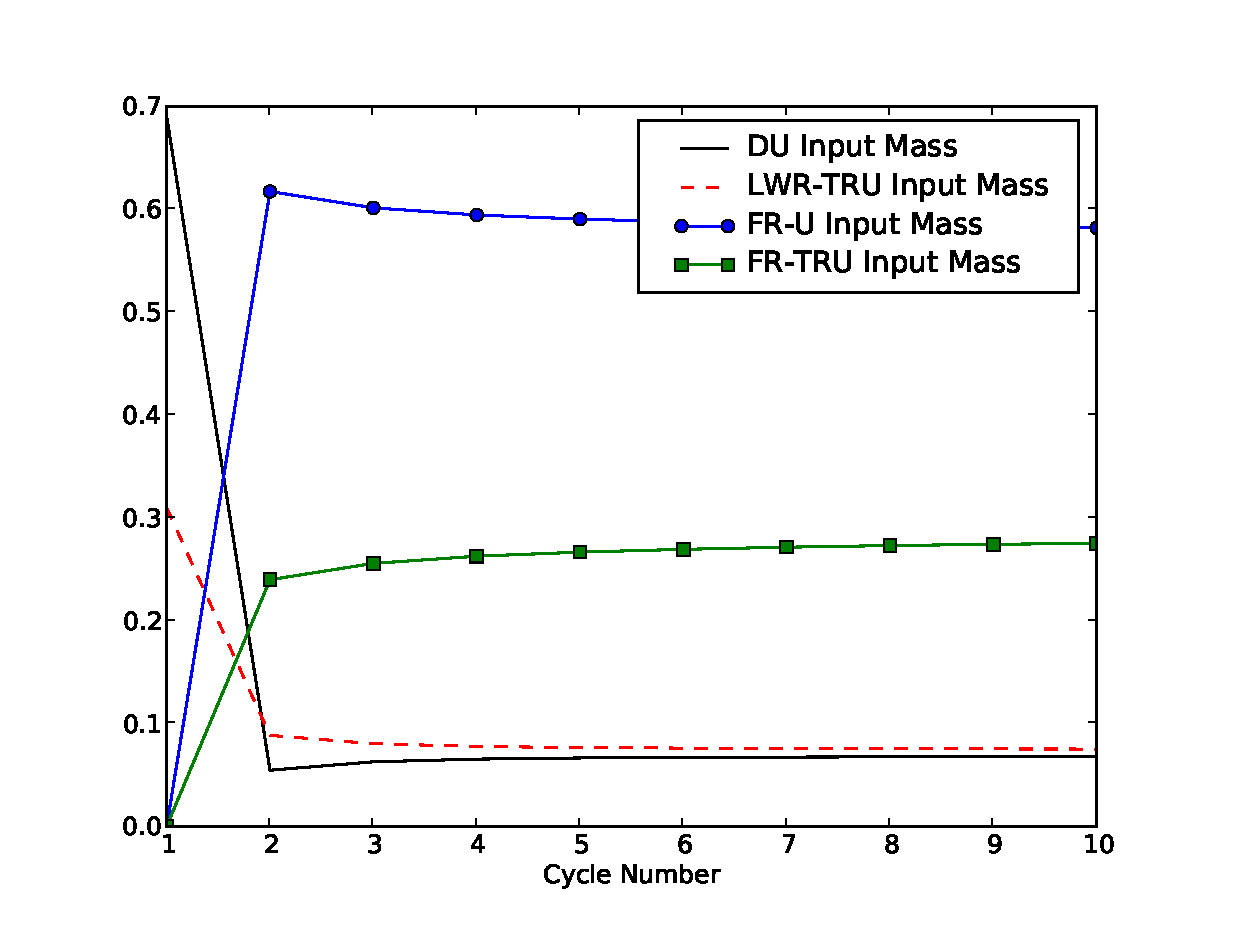
\includegraphics[scale=0.4]{../se_sensitivity/figs/MassStreams.eps}
\end{figure}
\end{center}
\end{slide}





% Fuel Cycle Dynamics
\begin{slide}{Fuel Cycle Dynamics}
\vspace{0.75cm}
\begin{center}
\begin{figure}
\caption{FR Output [kg/kgd] \& TRU CR}
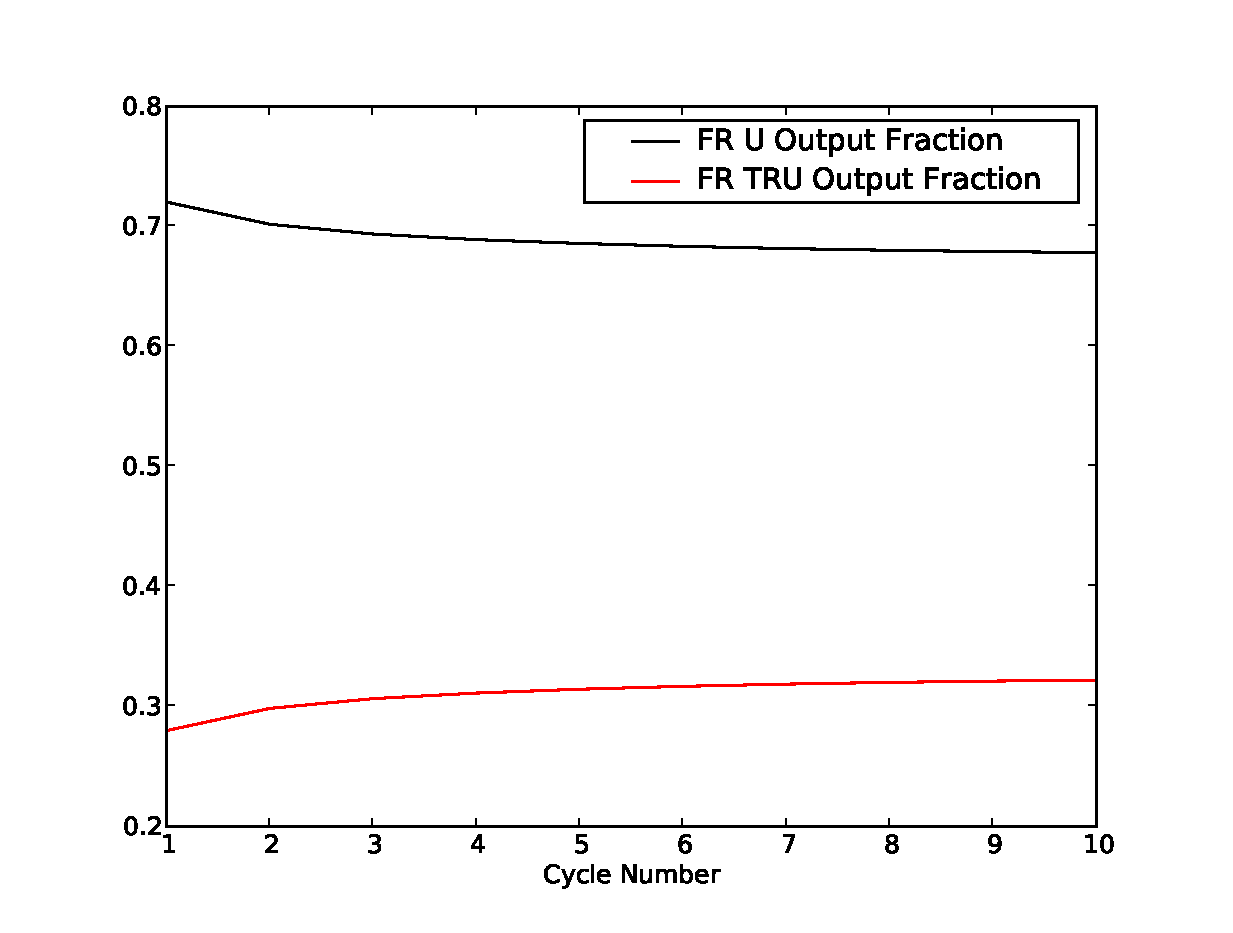
\includegraphics[scale=0.275]{../se_sensitivity/figs/FRfracOut.eps} 
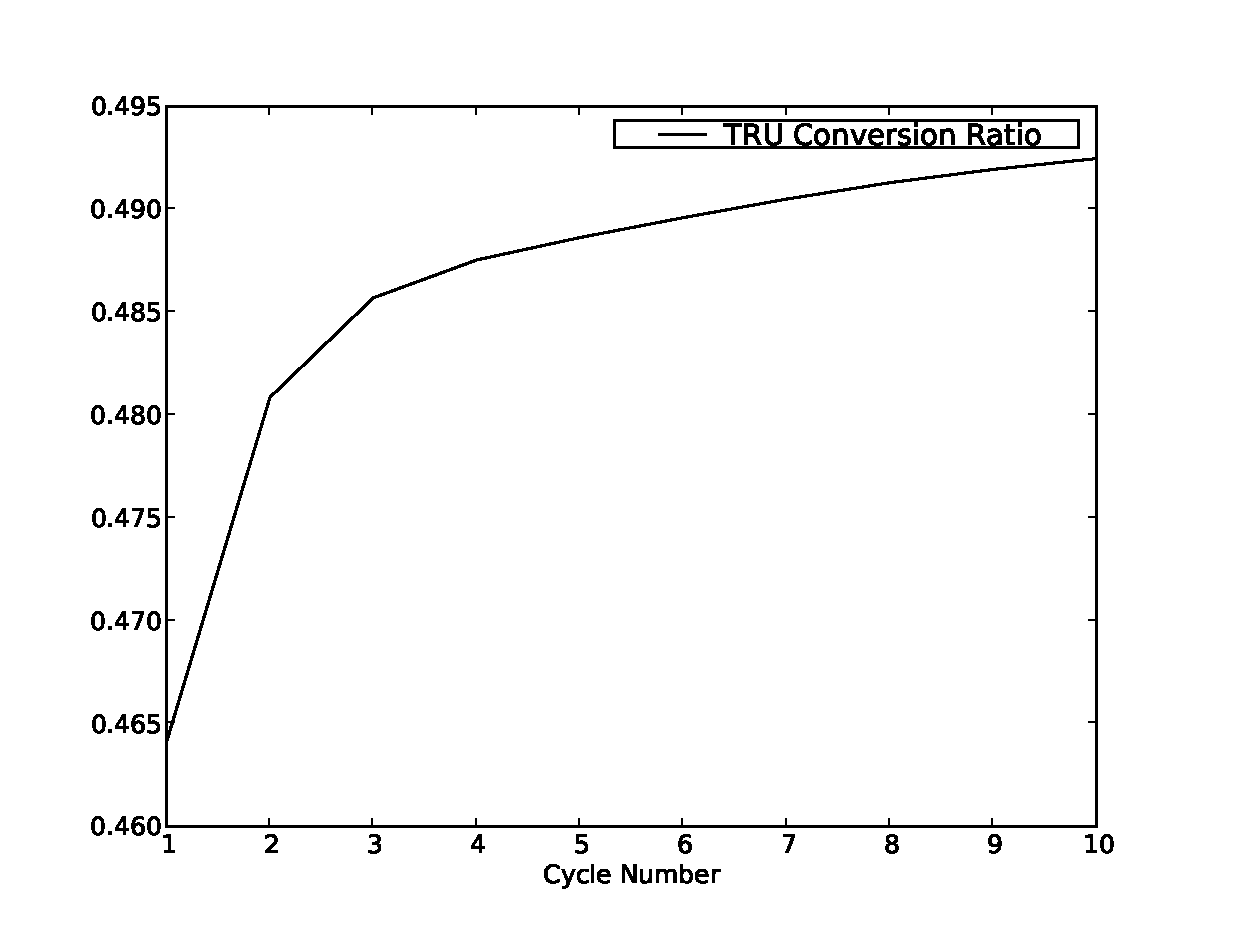
\includegraphics[scale=0.275]{../se_sensitivity/figs/TruCR.eps}
\end{figure}
\end{center}
\end{slide}




% Fuel Cycle Dynamics
\begin{slide}{Fuel Cycle Dynamics}
\vspace{0.75cm}
\begin{center}
\begin{figure}
\caption{\nuc{Np}{237}, \nuc{Pu}{239} Input and Output [kg/kgIHM]}
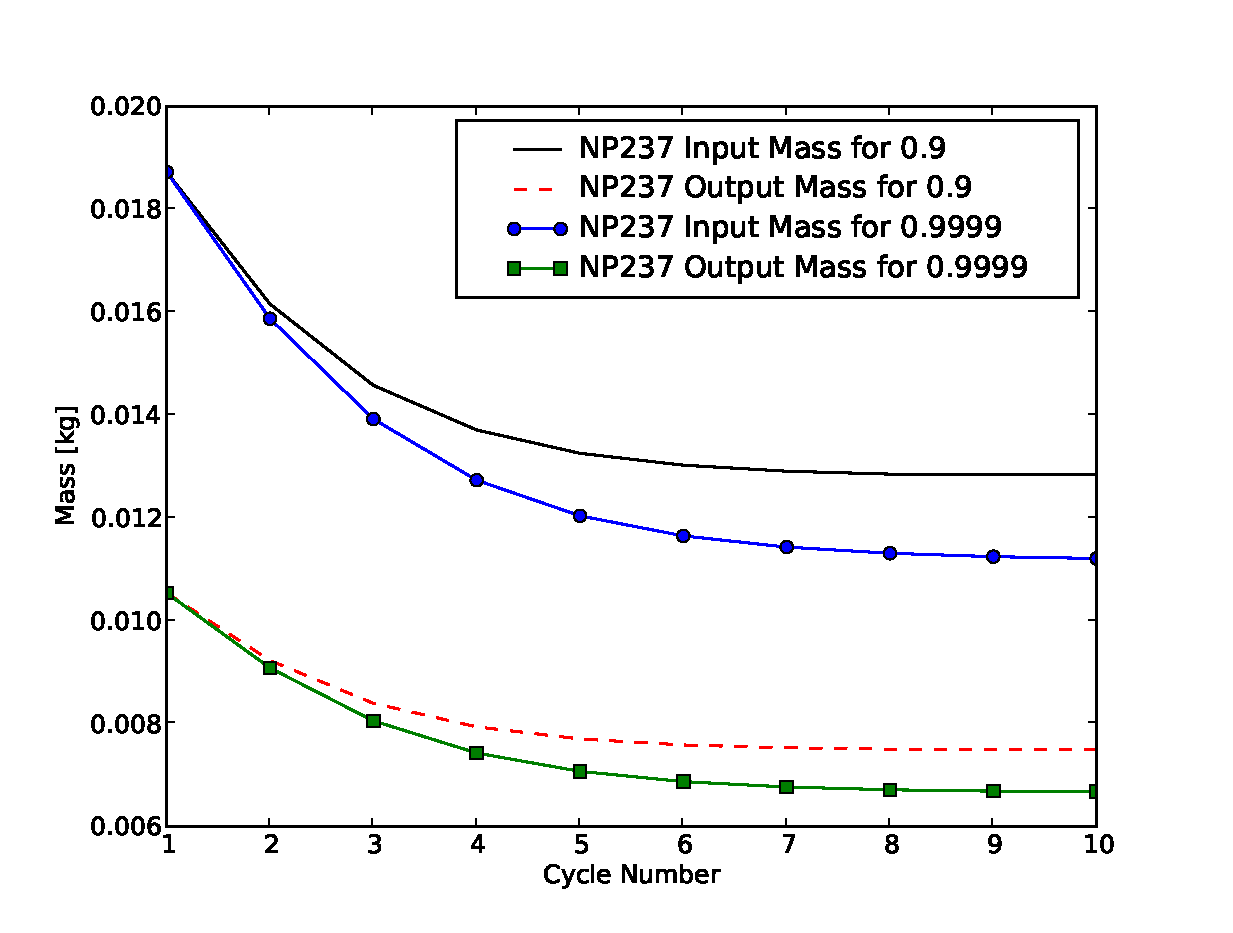
\includegraphics[scale=0.275]{../se_sensitivity/figs/NP237InOutSepEff.eps} 
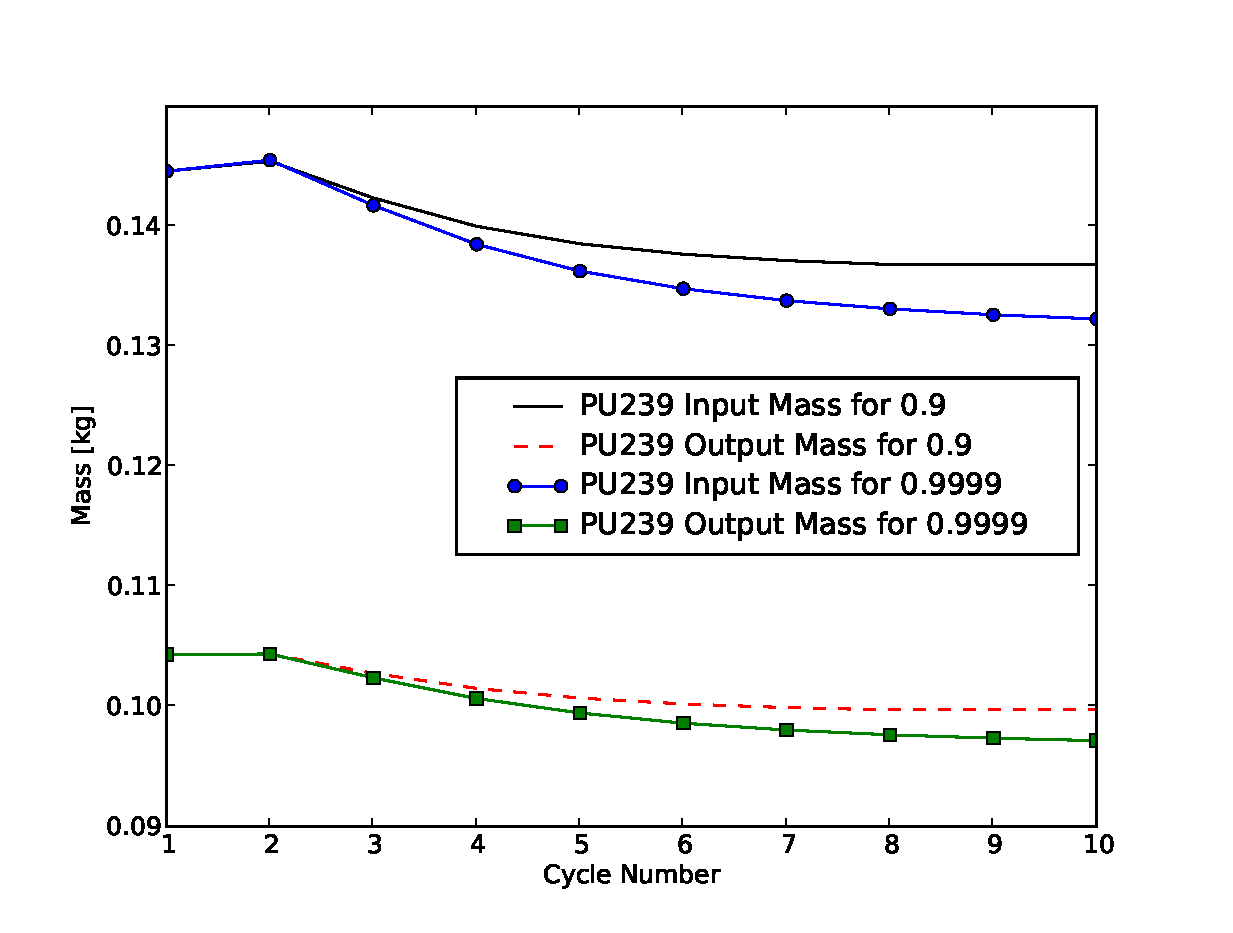
\includegraphics[scale=0.275]{../se_sensitivity/figs/PU239InOutSepEff.eps}
\end{figure}
\end{center}
\end{slide}




% Fuel Cycle Dynamics
\begin{slide}{Fuel Cycle Dynamics}
\vspace{0.75cm}
\begin{center}
\begin{figure}
\caption{\nuc{Am}{241}, \nuc{Cm}{244} Input and Output [kg/kgIHM]}
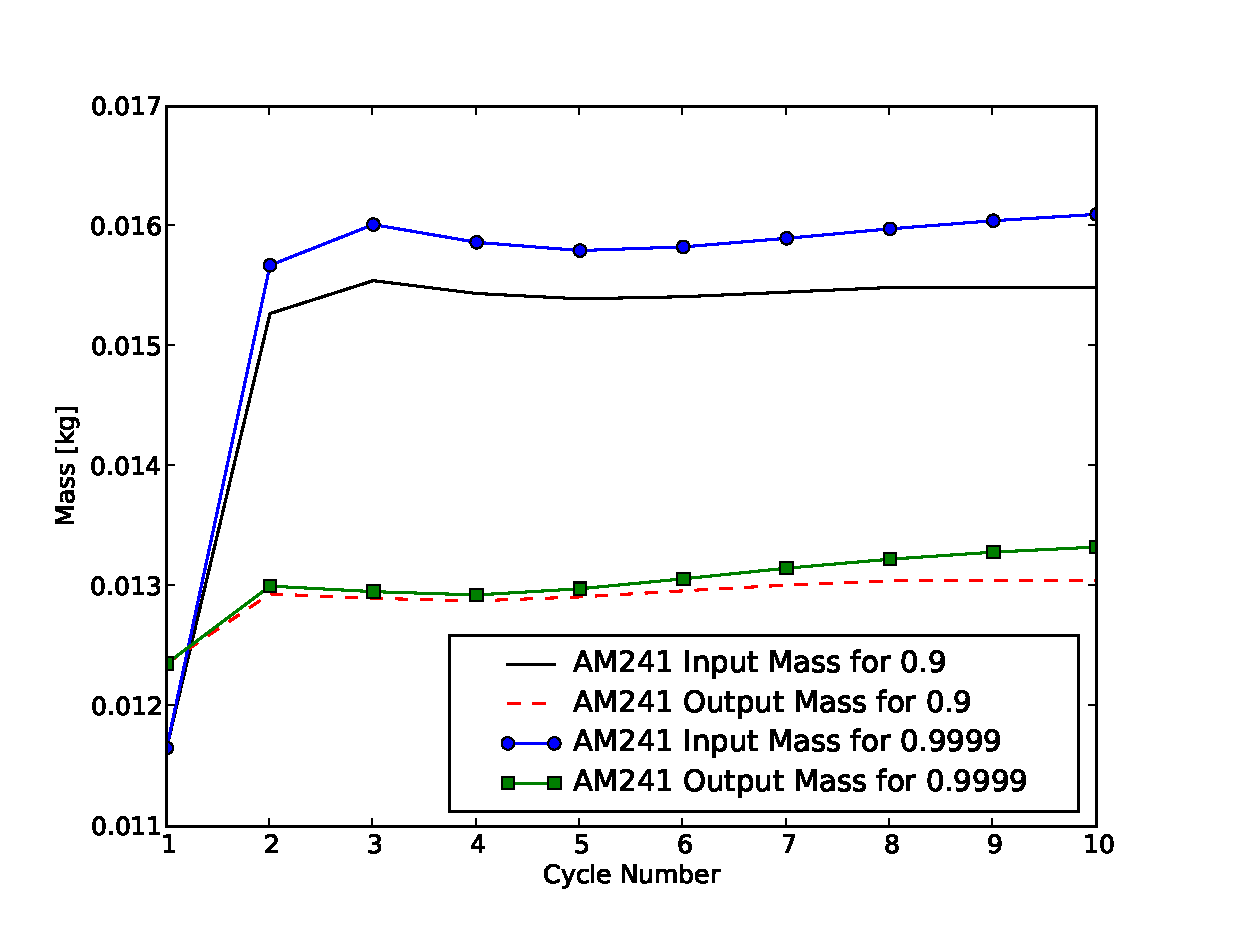
\includegraphics[scale=0.275]{../se_sensitivity/figs/AM241InOutSepEff.eps} 
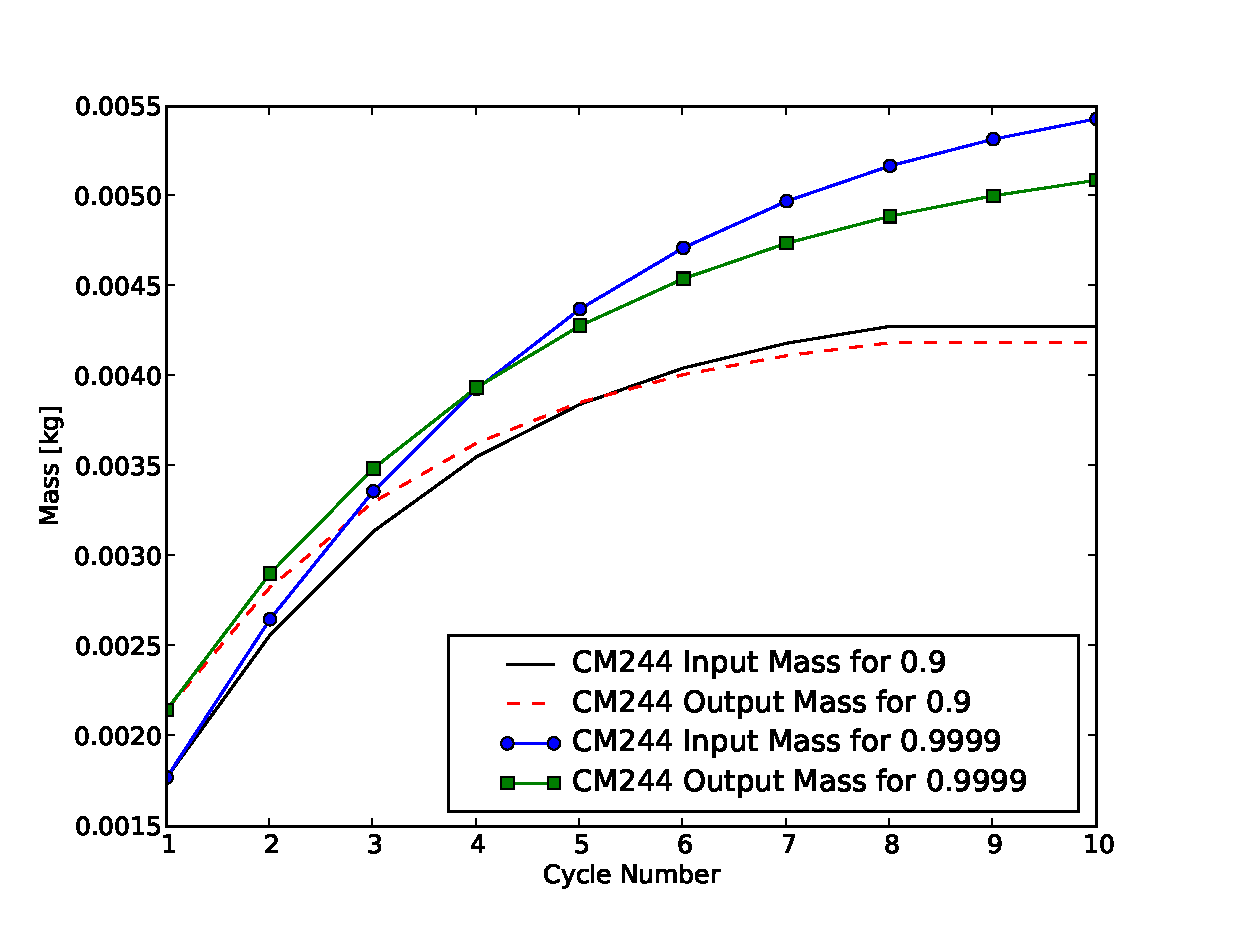
\includegraphics[scale=0.275]{../se_sensitivity/figs/CM244InOutSepEff.eps}
\end{figure}
\end{center}
\end{slide}




% Sensitivity Results
\begin{slide}{Sensitivity Results}
\begin{center}
\begin{table}
\scriptsize
\caption{Top Parameters from Screening Study}
\begin{tabular}{|l|c|c|c|}
\hline
\textbf{Parameter $x$}        & \textbf{Base Case $x_0$}    & \textbf{$S_{-x}$} [\%] & \textbf{$S_{+x}$} [\%]\\
\hline
\Red{\texttt{FR\_SE\_PU}}     & \Red{0.999}                 & \Red{-83.09}      & \Red{+99.30} \\
\hline
\Red{\texttt{LWR\_SE\_PU}}    & \Red{0.999}                 & \Red{-60.90}      & \Red{+18.28} \\
\hline
\Red{\texttt{FR\_SE\_AM}}     & \Red{0.999}                 & \Red{-59.53}      & \Red{+17.55} \\
\hline
\Red{\texttt{FR\_SE\_CM}}     & \Red{0.999}                 & \Red{-11.15}      & \Red{+1.28}  \\
\hline
\texttt{FR\_TRU\_CR}          & 0.500                       & +5.22             & -6.02  \\
\hline
\texttt{Rock\_Density}        & 2580 [kg/m\superscript{3}]  & -5.05             & +5.59  \\
\hline
\texttt{Rock\_Specific\_Heat} & 840 [J/kg/K]                & -4.90             & +5.59  \\
\hline
\texttt{LWR\_BUd}             & 50 [MWd/kg]                 & +5.46             & -3.48  \\
\hline
\texttt{FR\_BUd}              & 140 [MWd/kg]                & -5.44             & +5.32  \\
\hline
\end{tabular}
\end{table}
\end{center}
\end{slide}






% Sensitivity Results
\begin{slide}{Sensitivity Results}
\begin{center}
\begin{table}
\scriptsize
\caption{Bottom Parameters from Screening Study}
\begin{tabular}{|l|c|c|c|}
\hline
\textbf{Parameter $x$}           & \textbf{Base Case $x_0$}    & \textbf{$S_{-x}$} [\%] & \textbf{$S_{+x}$} [\%]\\
\hline
\Red{\texttt{LWR\_SE\_U}}        & \Red{0.999}                 & \Red{-0.01}      & \Red{+0.00} \\
\hline
\Red{\texttt{FR\_SE\_NP}}        & \Red{0.999}                 & \Red{-0.10}      & \Red{+0.01} \\
\hline
\Red{\texttt{FR\_SE\_U}}         & \Red{0.999}                 & \Red{-0.22}      & \Red{+0.01} \\
\hline
\texttt{FR\_LAN\_FF\_Cap}        & 0.0005 [w/o]                & +0.03            & -0.03 \\
\hline
\Red{\texttt{LWR\_SE\_NP}}       & \Red{0.999}                 & \Red{-0.26}      & \Red{+0.03} \\
\hline
\texttt{LWR\_SNF\_Storage\_Time} & 6 [y]                       & +0.06            & -0.14 \\
\hline
\Red{\texttt{LWR\_SE\_CM}}       & \Red{0.999}                 & \Red{-0.82}      & \Red{+0.08} \\
\hline
\texttt{Vent\_System\_On\_Time}  & 50 [y]                      & -0.11            & +1.13 \\
\hline
\texttt{Drift\_Diameter}         & 5.5 [m]                     & +0.26            & +0.58 \\
\hline
\end{tabular}
\end{table}
\end{center}
\end{slide}






%Counterintuitive Results
\overlays{5}{
\begin{slide}{Counterintuitive Results}
\FromSlide{1}
\begin{itemize}
    \item For drift diameter, both $S_{-x}$ and $S_{+x}$ are positive!

\vspace{0.2cm}
\FromSlide{2}
        \begin{itemize}
            \item This arises from the assumption that the dirft diameter very small as compared to the spacing 
                between drifts.
        \end{itemize}

\vspace{0.2cm}
\FromSlide{3}
    \item Since the base-case sits near a local drift diameter minimum, linear sensitivities will never 
        capture the full effect on the response.
    
\vspace{0.2cm}
\FromSlide{4}
    \item Additionally egregious is that, with increasing LWR burnup, the repository capacity goes down!

\vspace{0.2cm}
\FromSlide{5}
        \begin{itemize}
    \item This due to the overall TRU production \emph{per unit energy produced from the LWRs} declining.
        \end{itemize}

\FromSlide{1}
\end{itemize}
\end{slide}}






% LWR Burnup Sensitivity}
\begin{slide}{LWR Burnup Sensitivity}
\begin{center}
\begin{figure}
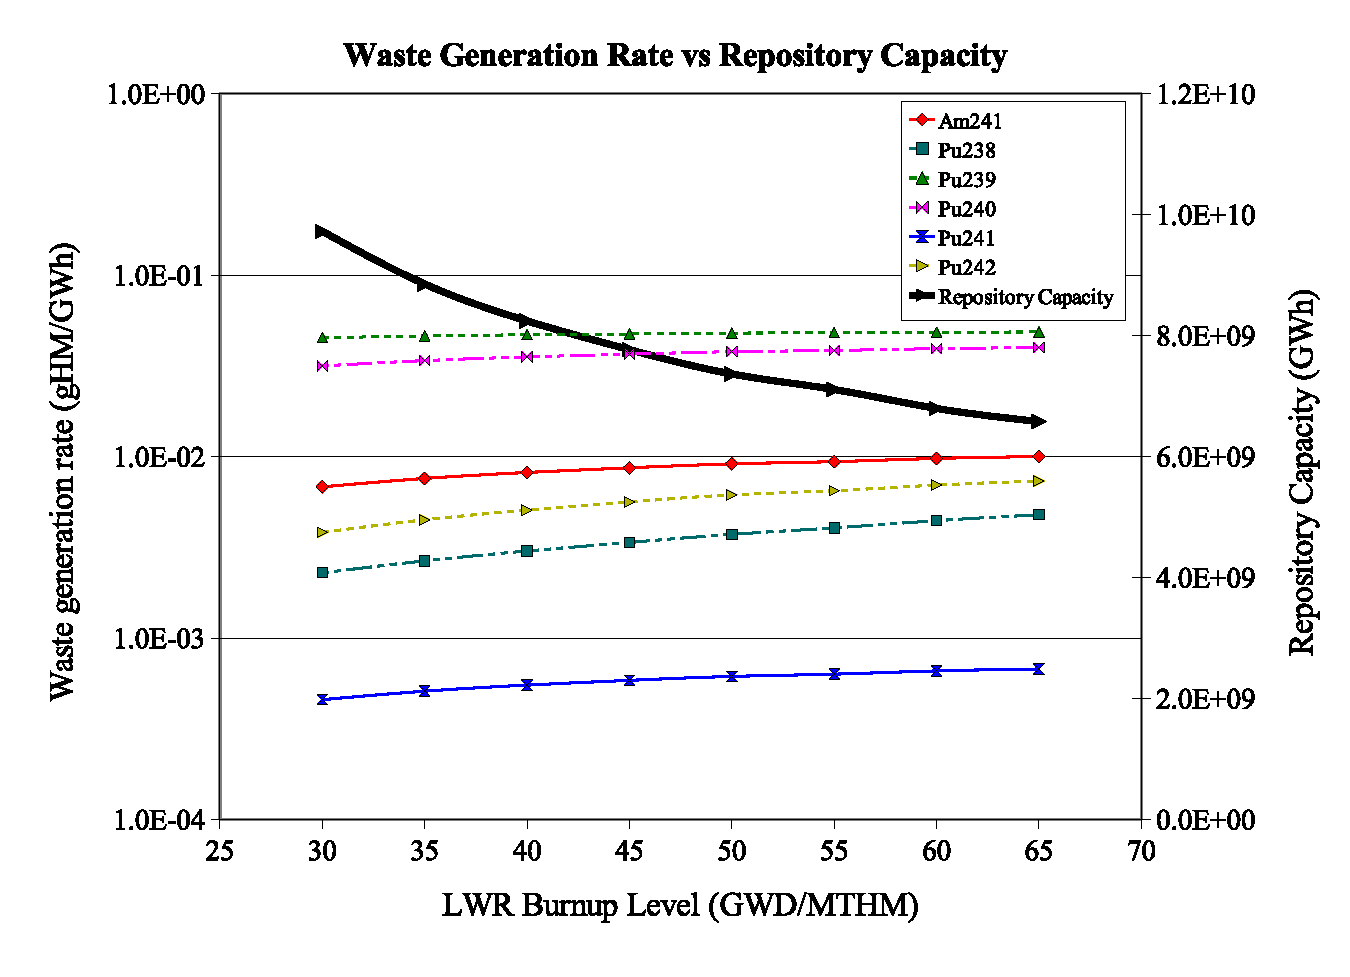
\includegraphics[scale=0.4]{figs/LWR_BUd_sensitivity_RepCap.eps}
\caption{Nuclide Generation Rate in the Final Waste}
\end{figure}
\end{center}
\end{slide}






%
% OMG next section
%

% Information Theoretic Fuel Cycle Analysis
\begin{slide}{Contingency Tables}
\vspace{3.5cm}
\begin{center}
\Large
Information Theoretic Analysis
\end{center}
\end{slide}





% Fuel Cycle Methodology
\overlays{4}{
\begin{slide}{Contingency Table Methodology}
\FromSlide{1}
\begin{itemize}
    \item Here again, the system-wide impact of physical parameter perturbations is quantified.

\FromSlide{2}
    \item This is done by performing \textbf{Contingency Table} analysis for each parameter
        to the \underline{repository} \underline{capacity} response.  

\FromSlide{3}
    \item Denote fuel cycle responses as $R$ [GWh] for $x$ \& $y$ input parameters.

\FromSlide{4}
    \item \textbf{\underline{Goal:}} Determine strength of \textit{association} 
        between inputs and pairs of inputs to the response in a manner that is independent to:
        \begin{itemize}
            \item the form of the response to the input $R(x)$,
            \item any base-case set of initial inputs.
        \end{itemize}

\FromSlide{1}
\end{itemize}
\end{slide}}




% Fuel Cycle Methodology
\begin{slide}{Contingency Table Methodology}
\begin{center}
\begin{figure}
\caption{Monte Carlo Methodology \& Analysis}
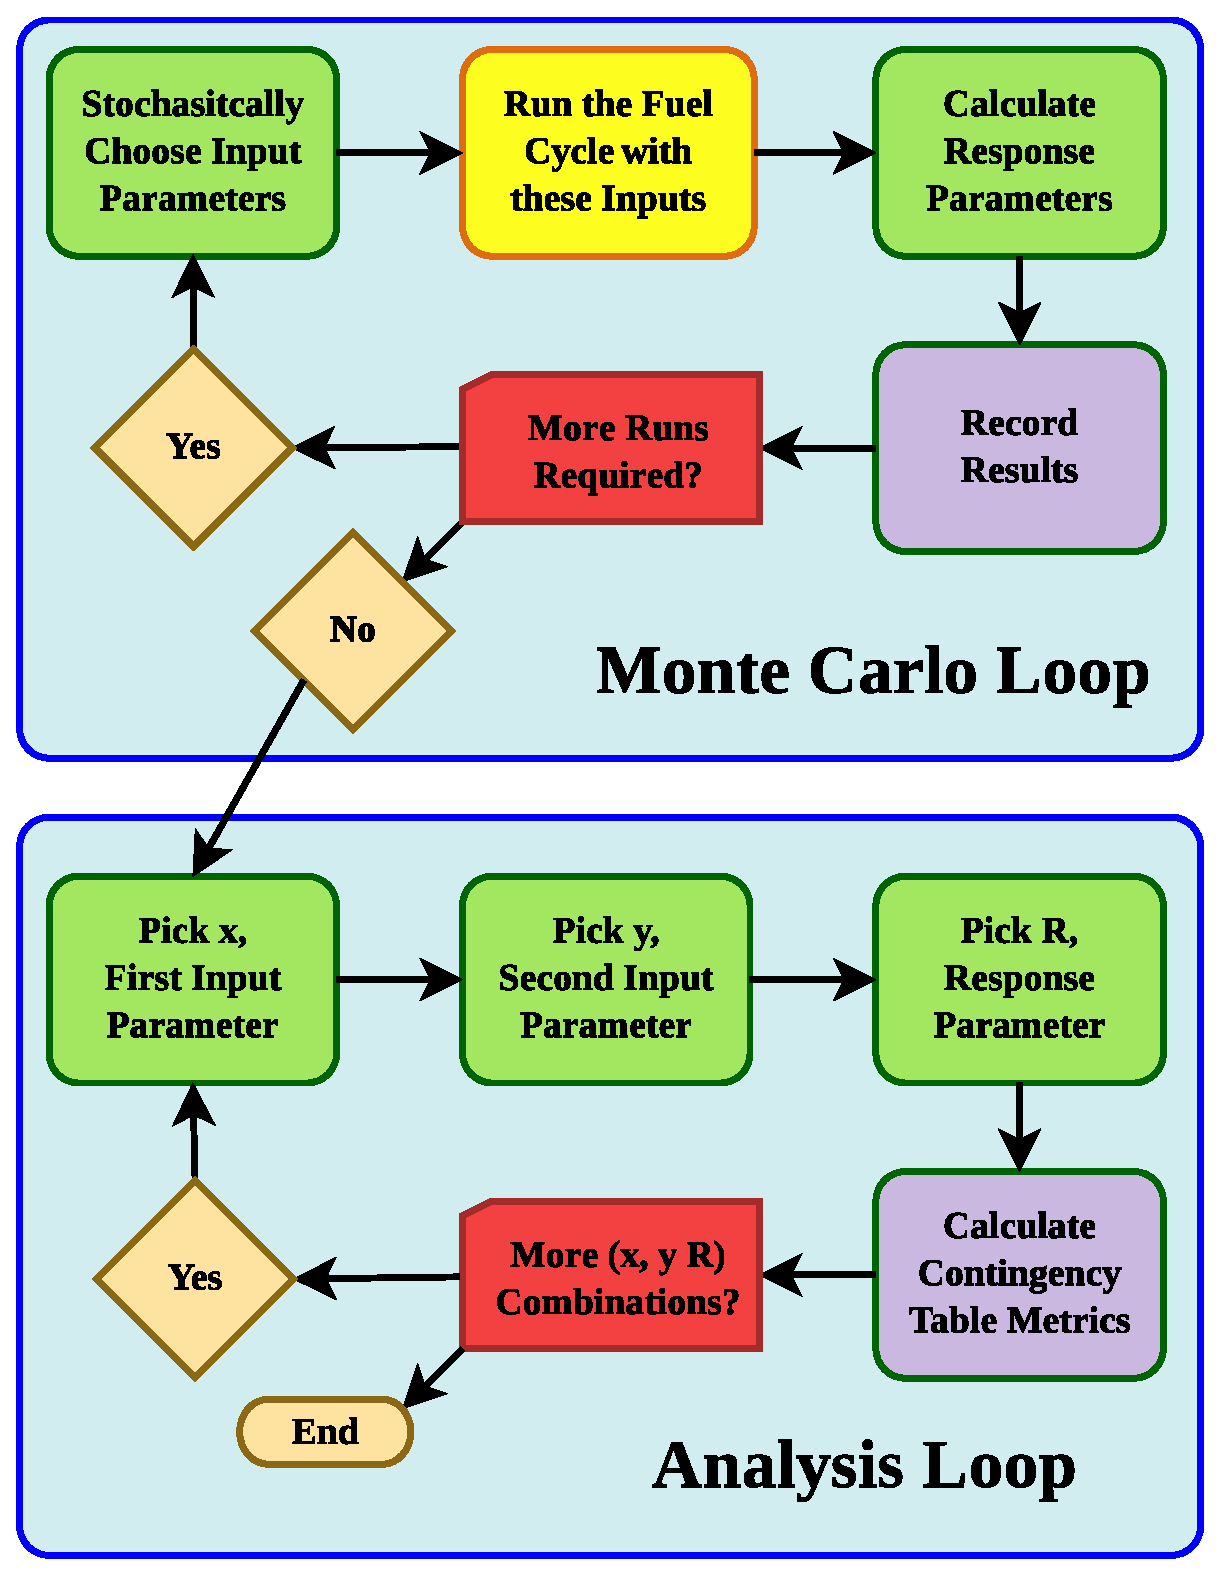
\includegraphics[scale=0.25]{../ct_sensitivity/figs/MonteCarloMethodology.eps}
\end{figure}
\end{center}
\end{slide}





% Input Parameter Definition
\begin{slide}{Input Parameter Definition}
\tiny
\begin{center}
\begin{tabular}{|l||c|c|c|c|}
\hline
\textbf{Input Parameter $x$} & \textbf{Min} & \textbf{Max} & \textbf{Units} & \textbf{Sample Type}\\
\hline
LWR Burnup Level & 30.0 & 80.0 & MWd/kgIHM & linear \\
\hline
LWR Fuel to Moderator Ratio & 0.28 & 0.36 & & linear \\
\hline
LWR SNF Storage Time & 3 & 30 & years & linear \\
\hline
SE of U from LWR UF & 0.99 & 0.9999 & & nines \\
\hline
SE of NP from LWR UF & 0.9 & 0.9999 & & nines \\
\hline
SE of PU from LWR UF & 0.9 & 0.9999 & & nines \\
\hline
SE of AM from LWR UF & 0.9 & 0.9999 & & nines \\
\hline
SE of CM from LWR UF & 0.9 & 0.9999 & & nines \\
\hline
SE of CS from LWR UF & 0.9 & 0.9999 & & nines \\
\hline
SE of SR from LWR UF & 0.9 & 0.9999 & & nines \\
\hline
FR Burnup Level & 100.0 & 200.0 & MWd/kgIHM & linear\\
\hline
FR TRU Conversion Ratio & 0.25 & 0.95 & & linear \\
\hline
Max Fraction of Lanthanide in FR Fuel & 0.0001 & 0.005 & Atoms/TRU Atom & linear \\
\hline
FR UF Storage Time & 3 & 30 & years & linear \\
\hline
Storage Before Disposal & 1 & 300 & years & log \\
\hline
\end{tabular}
\end{center}
\end{slide}

%Input Parameter Definition
\begin{slide}{Input Parameter Definition}
\tiny
\begin{center}
\begin{tabular}{|l||c|c|c|c|}
\hline
\textbf{Input Parameter $x$} & \textbf{Min} & \textbf{Max} & \textbf{Units} & \textbf{Sample Type}\\
\hline
SE of U from FR UF & 0.99 & 0.9999 & & nines \\
\hline
SE of NP from FR UF & 0.9 & 0.9999 & & nines \\
\hline
SE of PU from FR UF & 0.9 & 0.9999 & & nines \\
\hline
SE of AM from FR UF & 0.9 & 0.9999 & & nines \\
\hline
SE of CM from FR UF & 0.9 & 0.9999 & & nines \\
\hline
SE of CS from FR UF & 0.9 & 0.9999 & & nines \\
\hline
SE of SR from FR UF & 0.9 & 0.9999 & & nines \\
\hline
Density of Host Rock & 2317 & 2869 & kg/m\superscript{3} & linear \\
\hline
Specific Heat of Host Rock & 590 & 1270 & J/kg-K & linear \\
\hline
Thermal Conductivity of Host Rock & 1.9204 & 3.2856 & W/m-K & linear \\
\hline
Heat Loss Factor During Ventilation  & 0.806 & 0.914 & & linear \\
\hline
Drift diameter & 4.5 & 6.5 & m & linear \\
\hline
Ventilation System On Time & 10 & 300 & years & log \\
\hline
Ambient Environment Temperature & 12.82 & 32.82 & C & linear \\
\hline
Distance Between Drifts & 56 & 106 & m & linear \\
\hline
\end{tabular}
\end{center}
\end{slide}






% Contingency Table Methodology
\overlays{5}{
\begin{slide}{Contingency Table Methodology}
\FromSlide{1}
\begin{itemize}
    \item Before attempting to comprehend the subtleties of a 30+ dimensional surface,  
        prudence demands a check to see if all 30 variables are \textit{really} needed...

\FromSlide{2}
    \begin{itemize}
        \item (Hint: probably not!)
    \end{itemize}

\FromSlide{3}
    \item Thus a quantitative ranking of the \emph{associations} of each input parameter 
        to the response is desired.  

\FromSlide{4}
    \begin{itemize}
        \item (Note that these associations do not imply a linear response!)
    \end{itemize}

\FromSlide{5}
    \item These rankings are obtained by borrowing an analysis tool that is often 
        used in Biology: \underline{Contingency Tables}.

\FromSlide{1}
\end{itemize}
\end{slide}}



% Contingency Tables
\overlays{3}{
\begin{slide}{Contingency Tables}
\FromSlide{1}
The $2\times 2$ table is most common:
\setcounter{table}{4}
\begin{center}
\begin{table}
\caption{Hair Color to Sex Contingency Table}
\begin{tabular}{|l||c|c||c|}
\hline
       & Blonde & Brunette & Totals \\
\hline
Female & 18     & 17       & 35 \\
\hline
Male   & 11     & 14       & 25 \\
\hline
Totals & 29     & 31       & 60 \\
\hline
\end{tabular}
\end{table}
\end{center} 

\FromSlide{2}
\vspace{0.5cm}
But doesn't this approach ignore the underlying biology?

\FromSlide{3}
\vspace{0.5cm}
\raggedleft{\LARGE \textit{Yes!}}
\end{slide}}



% Contingency Tables
\overlays{6}{
\begin{slide}{Contingency Tables}
\begin{center}
\onlySlide*{1}{
\includegraphics[scale=0.125]{figs/CTBlackBox/CTBlackBox01.eps}}

\onlySlide*{2}{
\includegraphics[scale=0.125]{figs/CTBlackBox/CTBlackBox02.eps}}

\onlySlide*{3}{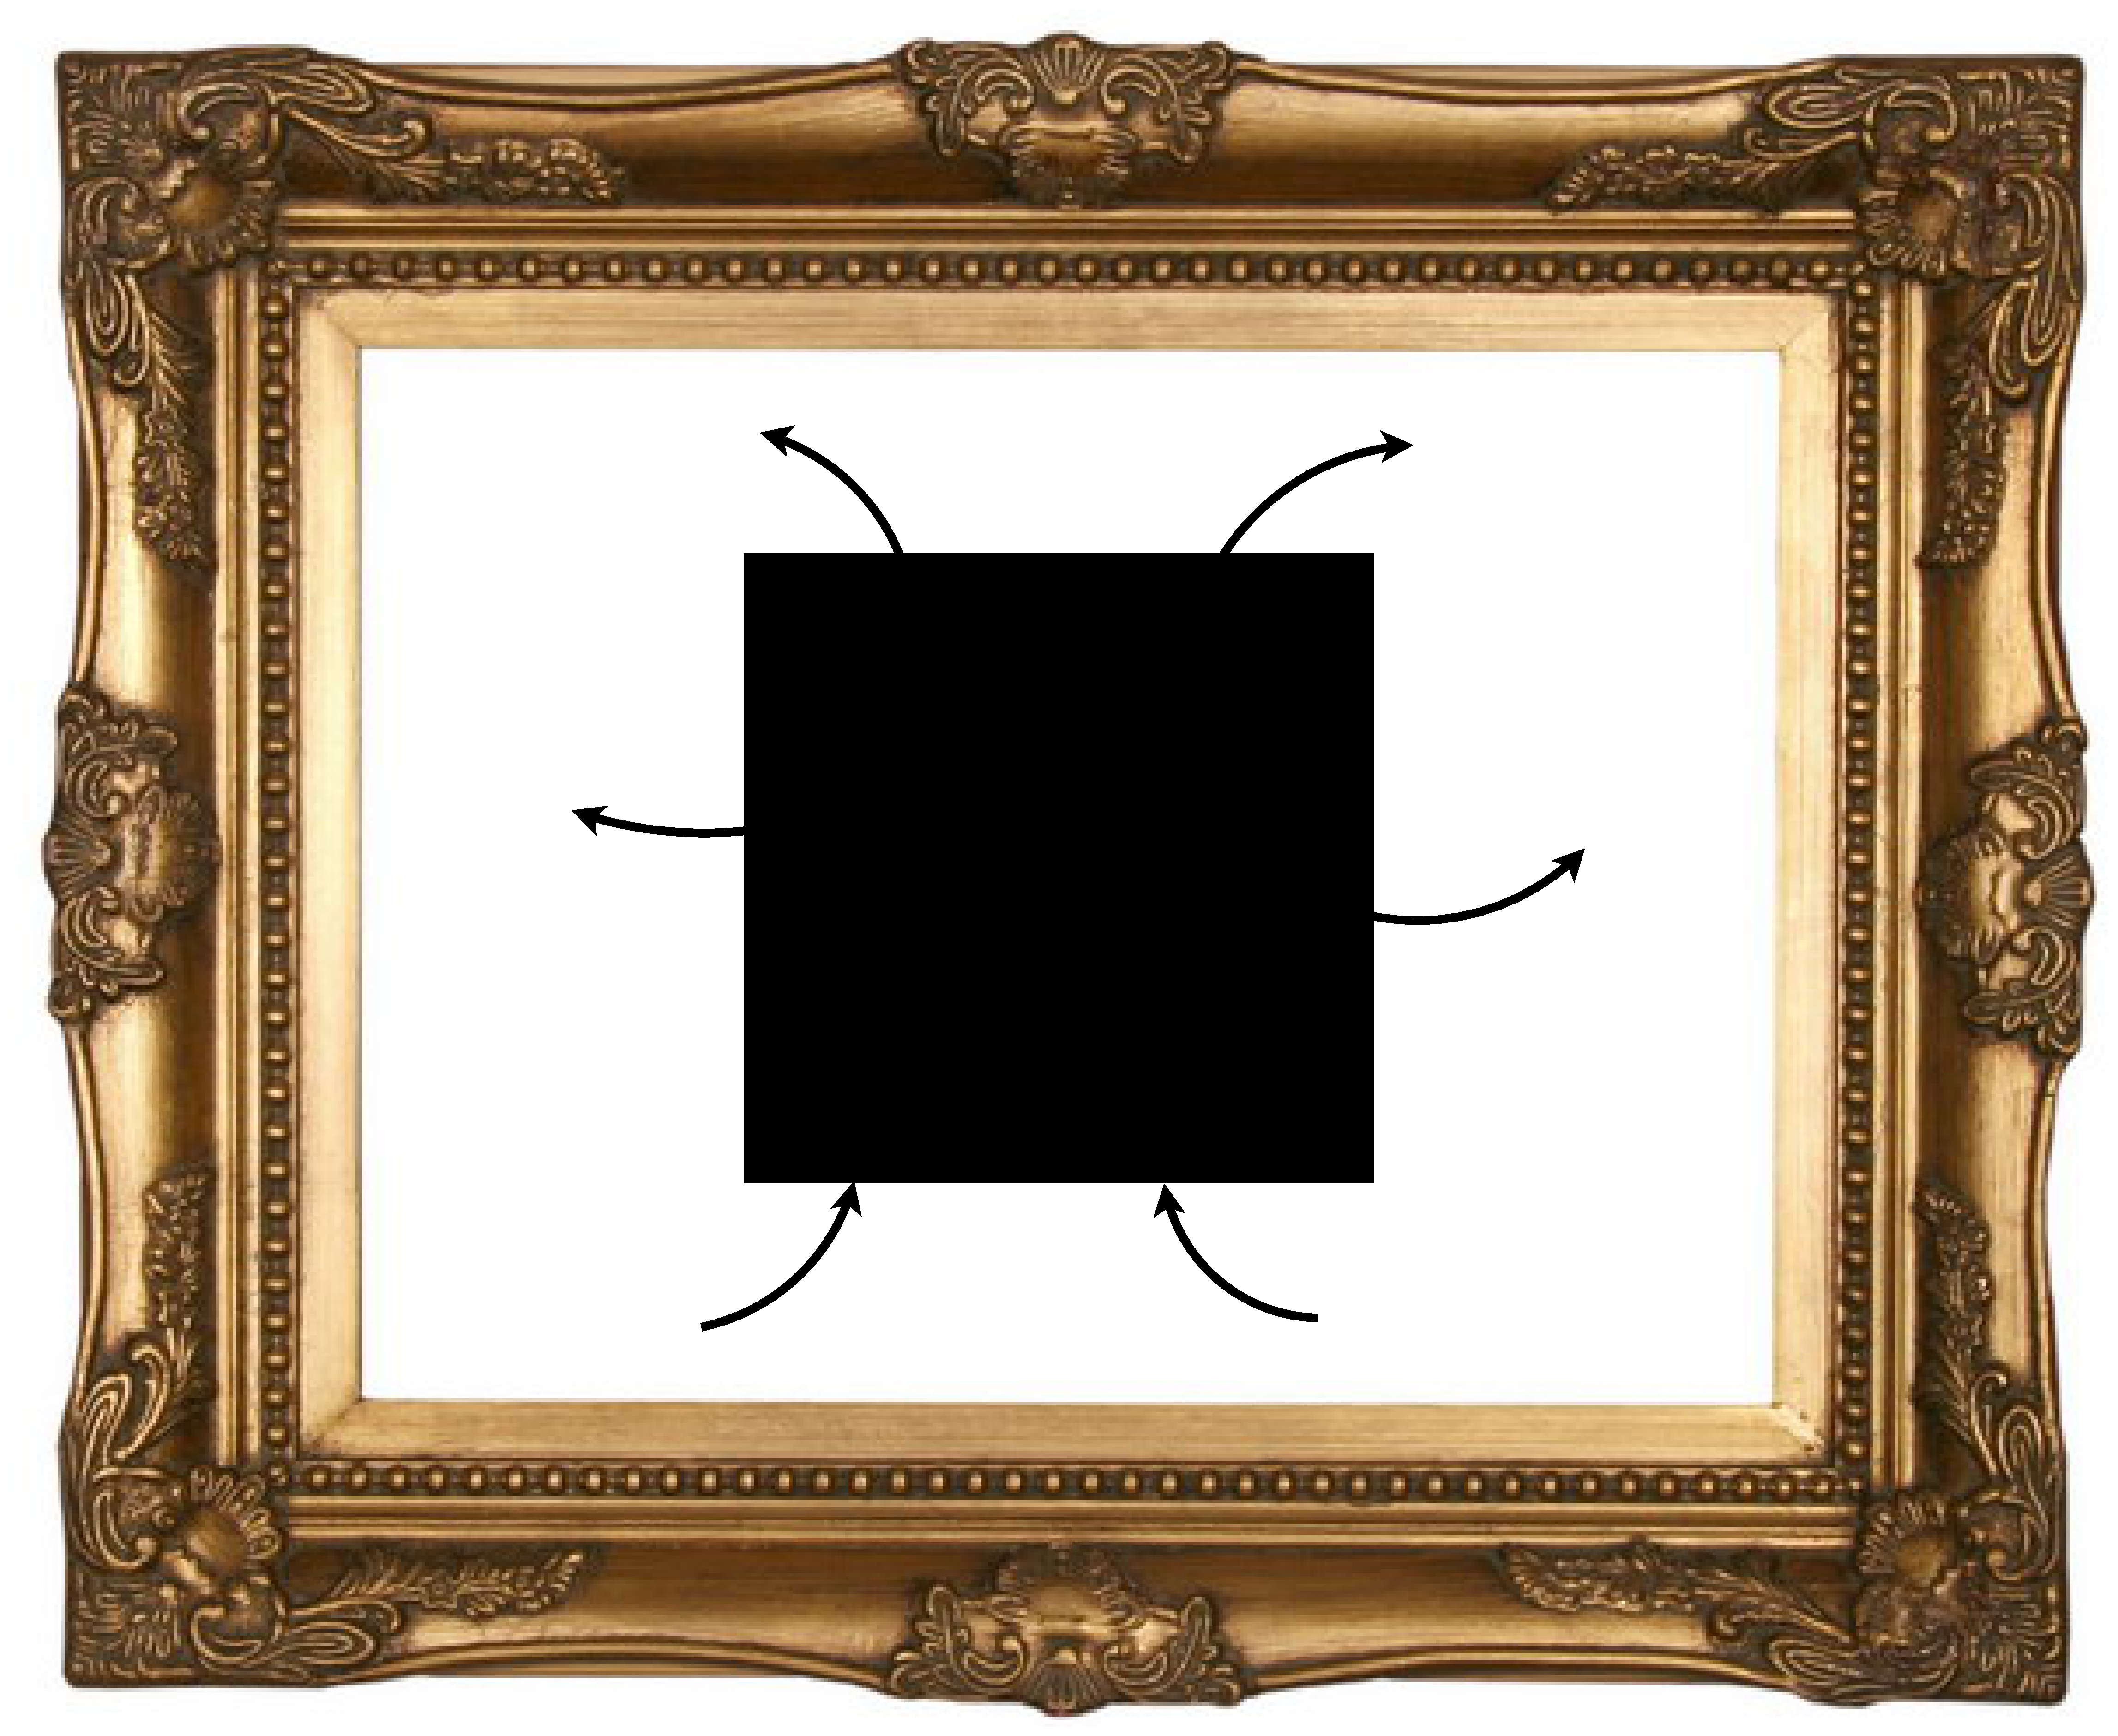
\includegraphics[scale=0.125]{figs/CTBlackBox/CTBlackBox03.eps}}

\onlySlide*{4}{
\includegraphics[scale=0.125]{figs/CTBlackBox/CTBlackBox04.eps}}

\onlySlide*{5}{
\includegraphics[scale=0.125]{figs/CTBlackBox/CTBlackBox05.eps}}

\onlySlide*{6}{
\includegraphics[scale=0.125]{figs/CTBlackBox/CTBlackBox06.eps}}
\end{center}
\end{slide}}



% Fuel Cycle Contingency Table
\overlays{2}{
\begin{slide}{Fuel Cycle Contingency Table}
\FromSlide{1}
For example, let's construct a 2D contingency table that 
measures the response from a sample input: fast reactor 
fuel plutonium separation efficiency, \texttt{FR\_SE\_PU}.

\FromSlide{2}
\vspace{0.50cm}
\begin{table}
\caption{Contingency Table for FR Plutonium SE to Repository Capacity [MTHM/Repository].}
\begin{center}
\footnotesize
\begin{tabular}{|c||c|c|c||c|}
\hline
&$0.9<$\texttt{SE}$<0.99$&$0.99<$\texttt{SE}$<0.999$&$0.999<$\texttt{SE}$<0.9999$&\\
\hline
$10^4 <$ \texttt{Capacity} $< 10^5$&$739$&$43$&$27$&$809$\\
\hline
$10^5 <$ \texttt{Capacity} $< 10^6$&$31510$&$21611$&$19469$&$72590$\\
\hline
$10^6 <$ \texttt{Capacity} $< 10^7$&$2648$&$13095$&$14430$&$30173$\\
\hline
$10^7 <$ \texttt{Capacity} $< 10^8$&$0$&$213$&$1053$&$1266$\\
\hline
&$34897$&$34962$&$34979$&$104838$\\
\hline
\end{tabular}
\end{center}
\label{ct2d_example}
\end{table}

\end{slide}}


% Contingency Table Statistics
\overlays{3}{
\begin{slide}{Contingency Table Statistics}
\FromSlide{1}
There are several metrics that have been developed to measure 
associations with contingency tables.  

\FromSlide{2}
\vspace{0.5cm}
The primary measure here is the \emph{Uncertainty Coefficient} $U(x|R)$.

\FromSlide{3}
\vspace{0.5cm}
To calculate $U(x|R)$ the following are needed, 
\begin{itemize}
    \item The \emph{Entropy} $H(x)$, which is a measure of how evenly the 
        data is spread out in the $x$ parameter.
    \item The \emph{Mutual Information} $I(R,x)$ which states the shared
        value of the $x$ together with $R$. 
\end{itemize}
\end{slide}}


% Contingency Table Statistics
\overlays{3}{
\begin{slide}{Contingency Table Statistics}
\FromSlide{1}
Denote the entries in a contingency table as $N_{ij}$ for the $i$\superscript{th} response bin
and the $j$\superscript{th} input bin.

\FromSlide{2}
\vspace{0.5cm}
The probability of landing in a given bin is therefore, 
\[ p_{ij} = \frac{N_{ij}}{N} \] 

\FromSlide{3}
\vspace{0.5cm}
Thus the entropy is calculated from, 
\[ H(x) = - \sum_j^J p_{\cdot j} \ln(p_{\cdot j}) \]
\end{slide}}


% Contingency Table Statistics
\overlays{2}{
\begin{slide}{Contingency Table Statistics}
\FromSlide{1}
The mutual information is found via, 
\[ I(R,x) = - \sum_{i,j}^{I,J} p_{ij} \ln\left(\frac{p_{ij}}{p_{i\cdot}\cdot p_{\cdot j}}\right) \]

\FromSlide{2}
\vspace{0.5cm}
The relations may be seen graphically [4]:

\vspace{0.5cm}
\setlength{\unitlength}{1cm}
\begin{center}
\begin{picture}(9,3)(-4.5,-1.5)
\thicklines
\put(0,1.5){\vector(1,0){4.5}}
\put(0,1.5){\vector(-1,0){4.5}}
\put(-0.7,1.2){\tiny $H(x,R)$}

\put(-2.25,1.0){\vector(1,0){2.25}}
\put(-2.25,1.0){\vector(-1,0){2.25}}
\put(-2.6,0.7){\tiny $H(x)$}

\put(1.5,0.5){\vector(1,0){3}}
\put(1.5,0.5){\vector(-1,0){3}}
\put(1.2,0.2){\tiny $H(R)$}

\put(-0.75,0){\vector(1,0){0.75}}
\put(-0.75,0){\vector(-1,0){0.75}}
\put(-1.2,-0.3){\tiny $I(R,x)$}

\put(-3,-0.5){\vector(1,0){1.5}}
\put(-3,-0.5){\vector(-1,0){1.5}}
\put(-3.5,-0.8){\tiny $H(x|R)$}

\put(2.25,-0.5){\vector(1,0){2.25}}
\put(2.25,-0.5){\vector(-1,0){2.25}}
\put(2.0,-0.8){\tiny $H(R|x)$}

\end{picture}
\end{center}

\end{slide}}


% Contingency Table Statistics
\overlays{2}{
\begin{slide}{Contingency Table Statistics}
\FromSlide{1}
The uncertainty coefficient is then calculated from,
\[ U(x|R) = \frac{I(R,x)}{H(x)} \]

\FromSlide{2}
This metric has the following useful properties:
\begin{enumerate}
    \item Defined on the range $[0, 1]$.
    \item $U(x|R) = 0$ implies that $I(R,x) = 0$, which indicates that the parameter
        is unassociated with the response.
    \item $U(x|R) = 1$ requires that $I(R,x) = H(x)$.  This implies that
        the system response $R(x)$ is solely determined by $x$.
\end{enumerate}
\end{slide}}



% Input Parameters Ranked by $U(x|R)$
\begin{slide}{Input Parameters Ranked by $U(x|R)$}
\begin{center}
\tiny
\begin{tabular}{|r|l|c|}
\hline
\textbf{Rank} & \textbf{$x$} & \textbf{$U(x|R)$}\\
\hline
1&\texttt{FR\_SE\_PU}&0.07667\\
\hline
2&\texttt{HLW\_Storage\_Time}&0.05264\\
\hline
3&\texttt{FR\_SE\_AM}&0.04148\\
\hline
4&\texttt{Heat\_Loss\_Factor}&0.01548\\
\hline
5&\texttt{LWR\_SE\_PU}&0.01343\\
\hline
6&\texttt{FR\_TRU\_CR}&0.008895\\
\hline
7&\texttt{LWR\_SE\_AM}&0.007304\\
\hline
8&\texttt{FR\_BUd}&0.003773\\
\hline
9&\texttt{LWR\_UF\_Storage\_Time}&0.003551\\
\hline
10&\texttt{Rock\_Specific\_Heat}&0.003085\\
\hline
11&\texttt{FR\_SE\_CM}&0.002522\\
\hline
12&\texttt{Rock\_Thermal\_Conductivity}&0.001954\\
\hline
13&\texttt{Ambient\_Temp}&0.001353\\
\hline
14&\texttt{LWR\_BUd}&0.001053\\
\hline
15&\texttt{LWR\_SE\_CS}&0.001033\\
\hline
\end{tabular}
\end{center}
\end{slide}



% Input Parameters Ranked by $U(x|R)$
\begin{slide}{Input Parameters Ranked by $U(x|R)$}
\begin{center}
\tiny
\begin{tabular}{|r|l|c|}
\hline
\textbf{Rank} & \textbf{$x$} & \textbf{$U(x|R)$}\\
\hline
16&\texttt{LWR\_SE\_SR}&0.001024\\
\hline
17&\texttt{FR\_UF\_Storage\_Time}&0.0005559\\
\hline
18&\texttt{Drift\_Space}&0.0004421\\
\hline
19&\texttt{LWR\_SE\_U}&0.0002899\\
\hline
20&\texttt{Rock\_Density}&0.0002718\\
\hline
21&\texttt{FR\_SE\_CS}&0.0001331\\
\hline
22&\texttt{FR\_SE\_SR}&0.0001073\\
\hline
23&\texttt{Vent\_System\_On\_Time}&0.0001016\\
\hline
24&\texttt{Drift\_Diameter}&9.648E-05\\
\hline
25&\texttt{LWR\_SE\_NP}&9.575E-05\\
\hline
26&\texttt{LWR\_SE\_CM}&7.969E-05\\
\hline
27&\texttt{LWR\_Fuel2Mod}&7.833E-05\\
\hline
28&\texttt{FR\_LAN\_FF\_Cap}&6.559E-05\\
\hline
29&\texttt{FR\_SE\_NP}&6.212E-05\\
\hline
30&\texttt{FR\_SE\_U}&6.207E-05\\
\hline
\end{tabular}
\end{center}
\end{slide}






% Contingency Table 3D Extension
\overlays{5}{
\begin{slide}{Contingency Table 3D Extension}
\FromSlide{1}
\begin{itemize}
    \item \textbf{\underline{New Goal:}} Now that the assoction of $x$ to $R$ may be determined, 
        finding the sensitivity of $R(x)$ to other inputs.

\FromSlide{2}
    \item Call $y$ an input parameter distinct from $x$.  Measuring the simultaneous
        effect of two inputs to a response may be performed using 3D tables!

\FromSlide{3}
    \item Note that \textit{`slices'} of these 3D tables may be seen as 2D tables bins 
        along a specific cut of data.

\FromSlide{4}
    \item For 30 inputs, there are $_{30}C_2 = 435$ contingency tables to construct.

\FromSlide{5}
    \item Different metrics will be needed to account for the added dimensionality.

\FromSlide{1}
\end{itemize}
\end{slide}}





% FR Pu SE and HLW Storage Time
\begin{slide}{FR Pu SE and HLW Storage Time}
\begin{center}
\tiny
\begin{tabular}{|c||c|c|c||c|}
\hline
\multicolumn{5}{|c|}{Slice for 1 $<$ \texttt{HLW\_Storage\_Time} $<$ 6.694}\\
\hline
&$0.9<$\texttt{SE}$<0.99$&$0.99<$\texttt{SE}$<0.999$&$0.999<$\texttt{SE}$< 0.9999$&\\
\hline
$10^4 <$ \texttt{Capacity} $< 10^5$&$419$&$23$&$14$&$456$\\
\hline
$10^5 <$ \texttt{Capacity} $< 10^6$&$11145$&$9970$&$9553$&$30668$\\
\hline
$10^6 <$ \texttt{Capacity} $< 10^7$&$110$&$1556$&$2085$&$3751$\\
\hline
$10^7 <$ \texttt{Capacity} $< 10^8$&$0$&$0$&$0$&$0$\\
\hline
&$11674$&$11549$&$11652$&$34875$\\
\hline
\hline
\multicolumn{5}{|c|}{Slice for 6.694 $<$ \texttt{HLW\_Storage\_Time} $<$ 44.814}\\
\hline
&$0.9<$\texttt{SE}$<0.99$&$0.99<$\texttt{SE}$<0.999$&$0.999<$\texttt{SE}$< 0.9999$&\\
\hline
$10^4 <$ \texttt{Capacity} $< 10^5$&$273$&$19$&$11$&$303$\\
\hline
$10^5 <$ \texttt{Capacity} $< 10^6$&$10859$&$7527$&$6373$&$24759$\\
\hline
$10^6 <$ \texttt{Capacity} $< 10^7$&$484$&$4157$&$5175$&$9816$\\
\hline
$10^7 <$ \texttt{Capacity} $< 10^8$&$0$&$2$&$24$&$26$\\
\hline
&$11616$&$11705$&$11583$&$34904$\\
\hline
\end{tabular}
\end{center}
\end{slide}




% FR Pu SE and HLW Storage Time
\begin{slide}{FR Pu SE and HLW Storage Time}
\begin{center}
\tiny
\begin{tabular}{|c||c|c|c||c|}
\hline
\multicolumn{5}{|c|}{Slice for 1 $<$ \texttt{HLW\_Storage\_Time} $<$ 6.694}\\
\hline
&$0.9<$\texttt{SE}$<0.99$&$0.99<$\texttt{SE}$<0.999$&$0.999<$\texttt{SE}$< 0.9999$&\\
\hline
$10^4 <$ \texttt{Capacity} $< 10^5$&$47$&$1$&$2$&$50$\\
\hline
$10^5 <$ \texttt{Capacity} $< 10^6$&$9506$&$4114$&$3543$&$17163$\\
\hline
$10^6 <$ \texttt{Capacity} $< 10^7$&$2054$&$7382$&$7170$&$16606$\\
\hline
$10^7 <$ \texttt{Capacity} $< 10^8$&$0$&$211$&$1029$&$1240$\\
\hline
&$11607$&$11708$&$11744$&$35059$\\
\hline
\hline
\multicolumn{5}{|c|}{Aggregation over \texttt{HLW\_Storage\_Time}}\\
\hline
&$0.9<$\texttt{SE}$<0.99$&$0.99<$\texttt{SE}$<0.999$&$0.999<$\texttt{SE}$< 0.9999$&\\
\hline
$10^4 <$ \texttt{Capacity} $< 10^5$&$739$&$43$&$27$&$809$\\
\hline
$10^5 <$ \texttt{Capacity} $< 10^6$&$31510$&$21611$&$19469$&$72590$\\
\hline
$10^6 <$ \texttt{Capacity} $< 10^7$&$2648$&$13095$&$14430$&$30173$\\
\hline
$10^7 <$ \texttt{Capacity} $< 10^8$&$0$&$213$&$1053$&$1266$\\
\hline
&$34897$&$34962$&$34979$&$104838$\\
\hline
\end{tabular}
\end{center}
\end{slide}





% 3D Contingency Table Statistics
\overlays{4}{
\begin{slide}{3D Contingency Table Statistics}
\FromSlide{1}
\begin{itemize}
    \item While $U(x,y|R)$ is roughly equivalent to the concept of \textit{mutual} \textit{sensitivity},
        3D tables should allow for an information theoretic parallel to \textit{\underline{covariance}}.

\FromSlide{2}
    \item In general for contingency tables covariance is not well defined, however here there is 
        the special stochastic situation where $x$ and $y$ are known \textit{a priori} to be independent of $R$.

\FromSlide{3}
    \item Therefore, the following new coefficient of variation metric is proposed:

\FromSlide{4}
        \begin{itemize}
            \item $c_v(x|y|R)$ is the \textit{`sensitivity of sensitivity'}, or how much an input 
                affects the response of another input.
        \end{itemize}

\FromSlide{1}
\end{itemize}
\end{slide}}





% 3D Contingency Table Statistics
\overlays{3}{
\begin{slide}{3D Contingency Table Statistics}
\FromSlide{1}
First, define:
\[ U(x|R)|y = \left\{ \left.U(x|R)\right|_{l_0}^{l_1}, \left.U(x|R)\right|_{l_1}^{l_2}, \ldots \left.U(x|R)\right|_{l_{C-1}}^{l_C}  \right\} \]

\FromSlide{2}
Then the coefficient of variation is,
\[ c_v(U(x|R)|y) = \frac{\sigma(U(x|R)|y)}{\mu(U(x|R)|y)} \]

\FromSlide{3}
Finally, the symmetric $c_v$ is set as:
\[ c_v(x|y|R) = \frac{1}{2} \left(c_v(U(x|R)|y) + c_v(U(y|R)|x)\right) \]
\end{slide}}



% 3D Contingency Table Statistics
\begin{slide}{3D Contingency Table Statistics}
\vspace{1.5cm}
Thus, $c_v(x|y|R)$ has the following properties:
\begin{enumerate}
    \item Defined on the range $[0, 1]$ since $0 \le U \le 1$.
    \item $c_v = 0$ implies that $\sigma = 0$, which indicates that $U(x|R)$
        shows no associaion with $y$.  Thus there are no covariant effects observed.
    \item $c_v = 1$ indicates that $\sigma = \mu$.  This connotes
        that the value of $x$ soley governs the response $R$ from $y$.
\end{enumerate}
\end{slide}





% $c_v(x|y|R)$ Parameter Pair Rankings
\begin{slide}{$c_v(x|y|R)$ Parameter Pair Rankings}
\begin{center}
\tiny
\begin{tabular}{|r|l|l|c|}
\hline
\textbf{Rank}&\textbf{$x$}&\textbf{$y$}&\textbf{$c_v(x|y|R)$}\\
\hline
1&\texttt{FR\_SE\_AM}&\texttt{HLW\_Storage\_Time}&0.02318\\
\hline
2&\texttt{FR\_SE\_AM}&\texttt{FR\_SE\_PU}&0.02316\\
\hline
3&\texttt{HLW\_Storage\_Time}&\texttt{LWR\_UF\_Storage\_Time}&0.01557\\
\hline
4&\texttt{FR\_SE\_PU}&\texttt{HLW\_Storage\_Time}&0.01556\\
\hline
5&\texttt{HLW\_Storage\_Time}&\texttt{LWR\_SE\_PU}&0.01155\\
\hline
6&\texttt{FR\_SE\_AM}&\texttt{FR\_TRU\_CR}&0.01061\\
\hline
7&\texttt{FR\_SE\_PU}&\texttt{LWR\_UF\_Storage\_Time}&0.008192\\
\hline
8&\texttt{FR\_SE\_PU}&\texttt{LWR\_SE\_PU}&0.008\\
\hline
9&\texttt{FR\_BUd}&\texttt{FR\_SE\_AM}&0.007716\\
\hline
10&\texttt{Ambient\_Temp}&\texttt{FR\_SE\_PU}&0.007489\\
\hline
11&\texttt{Ambient\_Temp}&\texttt{HLW\_Storage\_Time}&0.007367\\
\hline
12&\texttt{HLW\_Storage\_Time}&\texttt{LWR\_SE\_AM}&0.007248\\
\hline
13&\texttt{Ambient\_Temp}&\texttt{FR\_SE\_CS}&0.007235\\
\hline
14&\texttt{Ambient\_Temp}&\texttt{LWR\_Fuel2Mod}&0.007066\\
\hline
15&\texttt{Ambient\_Temp}&\texttt{Heat\_Loss\_Factor}&0.007044\\
\hline
\end{tabular}
\end{center}
\end{slide}






% Parameter Pair Example
\begin{slide}{Parameter Pair Example}
\begin{center}
\begin{figure}
\caption{Total \& Top Contributors to Decay Heat [Watts/kg] of HLW for (\texttt{FR\_SE\_AM}, \texttt{FR\_SE\_PU}).}
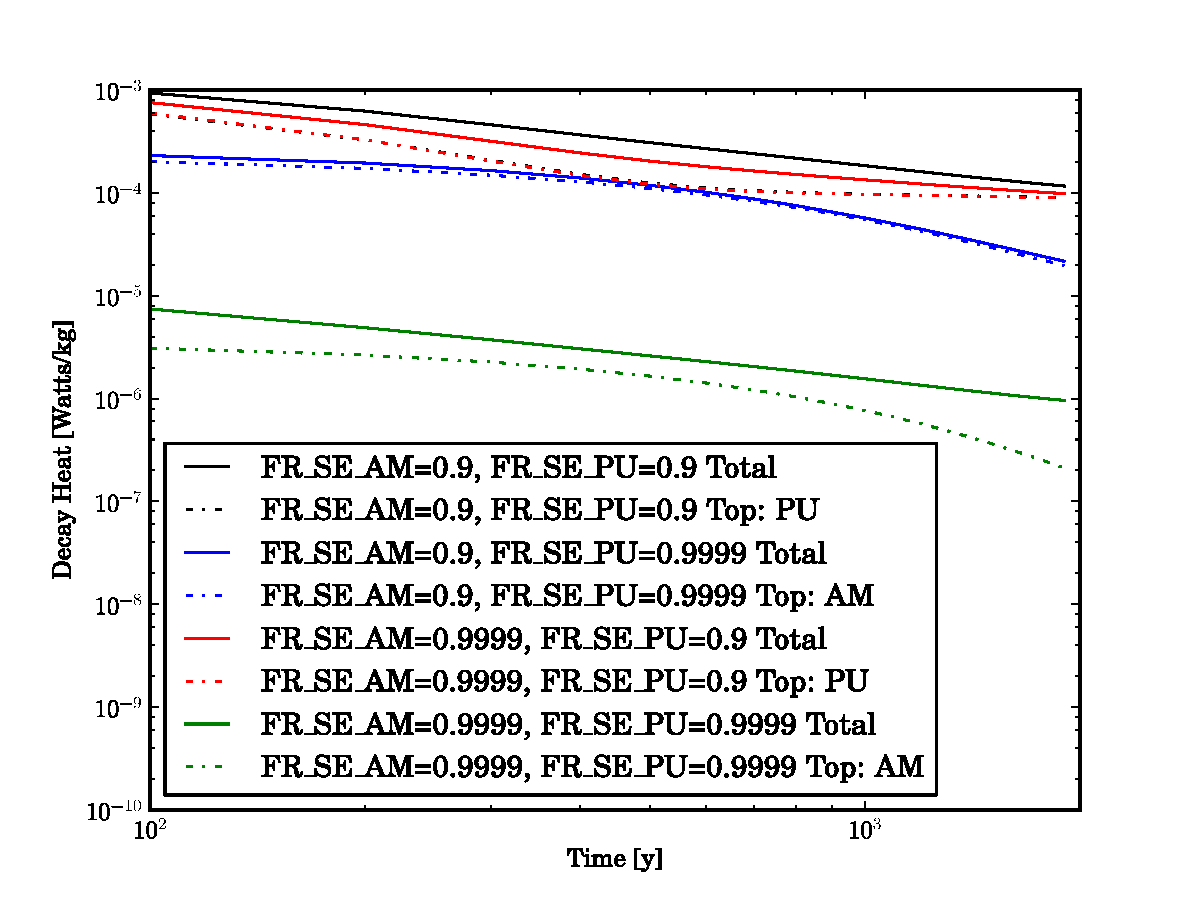
\includegraphics[scale=0.375]{../ct_sensitivity/figs/FR_SE_AM_and_FR_SE_PU_Decay_Heat.eps}
\end{figure}
\end{center}
\end{slide}




%
% OMG next section
%

% RMG
\begin{slide}{RMG}
\vspace{3.5cm}
\begin{center}
\Large
Multi-Group Reactor Model
\end{center}
\end{slide}




% Remotivation
\overlays{3}{
\begin{slide}{Remotivation}
\FromSlide{1}
\begin{itemize}
    \item In the R1G, fluxes are assumed to be static over the course of the burn.

    \FromSlide{2}
    \vspace{1cm}
    \begin{itemize}
        \item This restricts the types of reactors and fuel cycles which may be modeled.
            (MOX, IMF, Traveling Wave, \emph{etc.} are unavailable to the R1G.)
    \end{itemize}

\FromSlide{3}
\vspace{1cm}
    \item Also in the R1G, changing reactor state variables in a way that would affect
        the flux spectrum required additional libraries, or inter-library interpolations.

\FromSlide{1}
\end{itemize}
\end{slide}}





% Remotivation
\overlays{3}{
\begin{slide}{Remotivation}
\FromSlide{1}
\begin{itemize}
    \item To solve these issues, moving to a multi-energy group reactor model 
        will enable automatic spectral shifts in the core as needed.

    \FromSlide{2}
    \vspace{0.75cm}
    \begin{itemize}
        \item Rather than prameterizing burnup, transmutation, and neutron 
            production \& destruction rates as functions of nuclide and fluence, 
            the RMG parameterizes cross sections over a number of different states.
    \end{itemize}

\FromSlide{3}
\vspace{0.75cm}
    \item The R1G parameters are explicitly solved for by the RMG model.

\FromSlide{1}
\end{itemize}
\end{slide}}







%Conclusions
\overlays{4}{
\begin{slide}{Conclusions}
\FromSlide{1}
\begin{itemize}
    \item We have demonstrated a quick fuel cycle methodology that passes 
        both unit and integral tests.

\FromSlide{2}
    \item Using this new tool, we have developed a robust alternative to simple fuel cycle 
        sensitivity studies using contingency tables and their related statistics.

\FromSlide{3}
    \item This methodology is both quantitative and independent of the functional form 
        between the input and response. 

\FromSlide{4}
    \item In fact, these new metrics do not even require that the stochastic variables 
        be sampled in the same way.


\FromSlide{1}
\end{itemize}
\end{slide}}










% Questions
\begin{slide}{Questions}
? ? ? ? ? ? ? ? ? ? ? ? ? ? ? ? ? ? ? ? ? ? ? ? ? ? ? ? ? ? ? 
? ? ? ? ? ? ? ? ? ? ? ? ? ? ? ? ? ? ? ? ? ? ? ? ? ? ? ? ? ? ? 
? ? ? ? ? ? ? ? ? ? ? ? ? ? ? ? ? ? ? ? ? ? ? ? ? ? ? ? ? ? ? 
? ? ? ? ? ? ? ? ? ? ? ? ? ? ? ? ? ? ? ? ? ? ? ? ? ? ? ? ? ? ? 
? ? ? ? ? ? ? ? ? ? ? ? ? ? ? ? ? ? ? ? ? ? ? ? ? ? ? ? ? ? ? 
? ? ? ? ? ? ? ? ? ? ? ? ? ? ? ? ? ? ? ? ? ? ? ? ? ? ? ? ? ? ? 
? ? ? ? ? ? ? ? ? ? ? ? ? ? ? ? ? ? ? ? ? ? ? ? ? ? ? ? ? ? ? 
? ? ? ? ? ? ? ? ? ? ? ? ? ? ? ? ? ? ? ? ? ? ? ? ? ? ? ? ? ? ? 
? ? ? ? ? ? ? ? ? ? ? ? ? ? ? ? ? ? ? ? ? ? ? ? ? ? ? ? ? ? ? 
? ? ? ? ? ? ? ? ? ? ? ? ? ? ? ? ? ? ? ? ? ? ? ? ? ? ? ? ? ? ? 
? ? ? ? ? ? ? ? ? ? ? ? ? ? ? ? ? ? ? ? ? ? ? ? ? ? ? ? ? ? ? 
? ? ? ? ? ? ? ? ? ? ? ? ? ? ? ? ? ? ? ? ? ? ? ? ? ? ? ? ? ? ? 
? ? ? ? ? ? ? ? ? ? ? ? ? ? ? ? ? ?
\end{slide}

\begin{slide}{Bibliography}
\tiny
\begin{enumerate}
    \item \fullcite{Scopatz2009}
    \item \fullcite{Takano1994}
    \item \fullcite{NEA-5990}
    \item \fullcite{Press2007c}
\end{enumerate}
\end{slide}

\end{document}
